\addtocontents{toc}{\protect\vspace{\beforebibskip}}% Place slightly below the rest of the document content in the table


%************************************************
\chapter{Desenvolvimento}
\label{ch:desenvolvimento}
%************************************************

\section{Teste 5}

\subsection{Objetivo}
Classificar Imagens com quadrados parciais e quadrados normais. É importante mencionar que os quadrados parciais estão todos com parte fora da imagem, nas extremidades. 

\subsection{Dataset}
O Dataset é composto por 11000 imagens de treino e 5000 de teste. Composto por 2 classes: 
\begin{itemize}
    \item Quadrados 
    \item Quadrados Parciais

\end{itemize}
\begin{figure}[H]
    \centering
    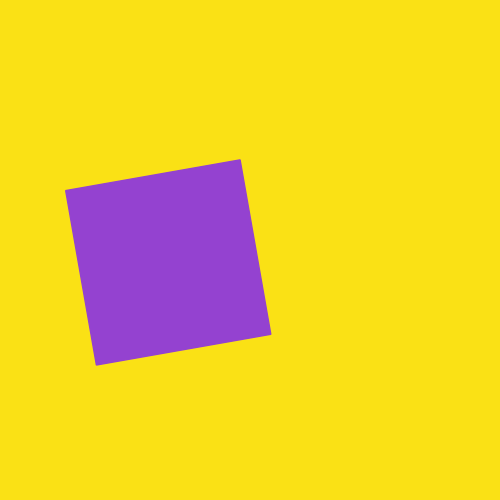
\includegraphics[width=0.35\linewidth]{imgs/Test_5/dataset_5/square_5501.png}
    
\includegraphics[width=0.35\linewidth]{imgs/Test_5/dataset_5/square_cut_5501.png}
    \caption{Quadrado e Quadrado Parcial}
    \label{fig:enter-label}
\end{figure}
\begin{figure}[H]
    \centering
    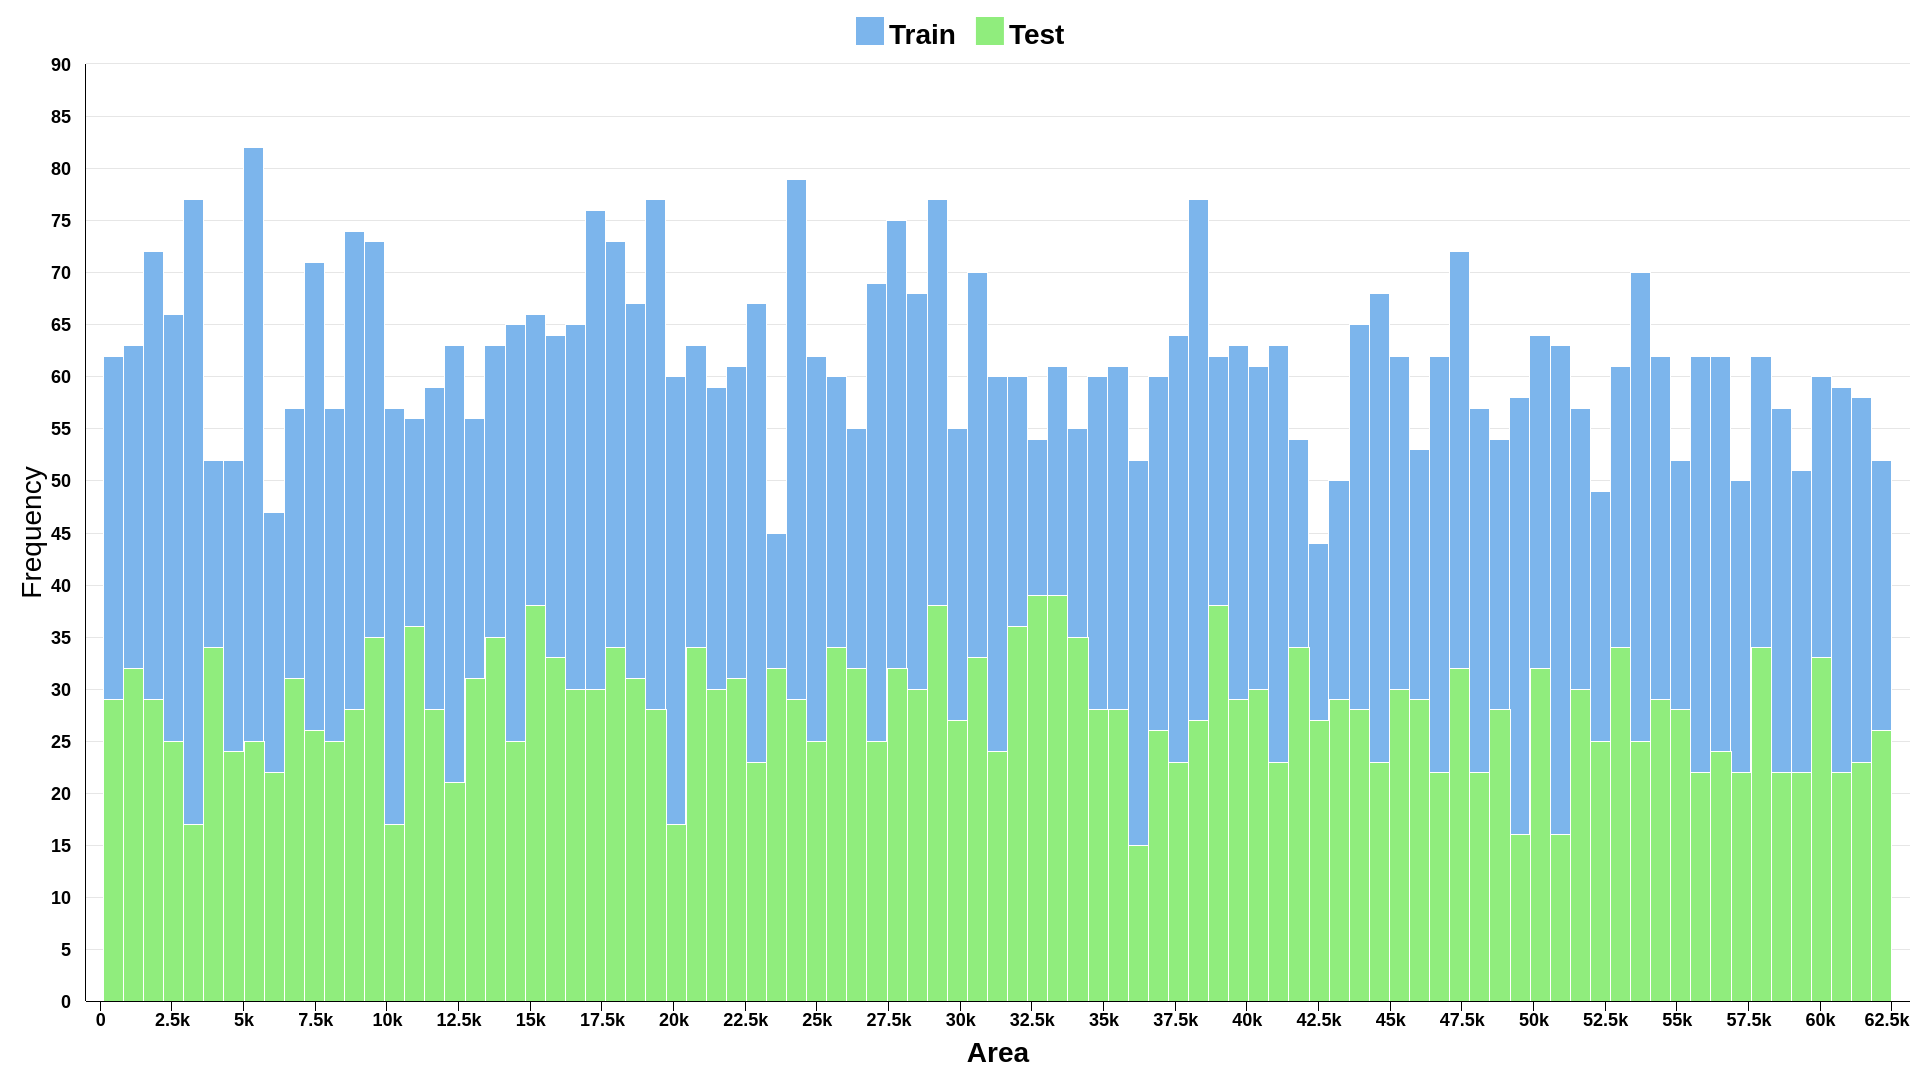
\includegraphics[width=1.0\linewidth]{imgs/Test_5/dataset_5/Squares_Area_Distribution_Hist.png}
    \caption{Distribuição da Área (Quadrados)}
    \label{fig:enter-label}
\end{figure}
\begin{figure}[H]
    \centering
    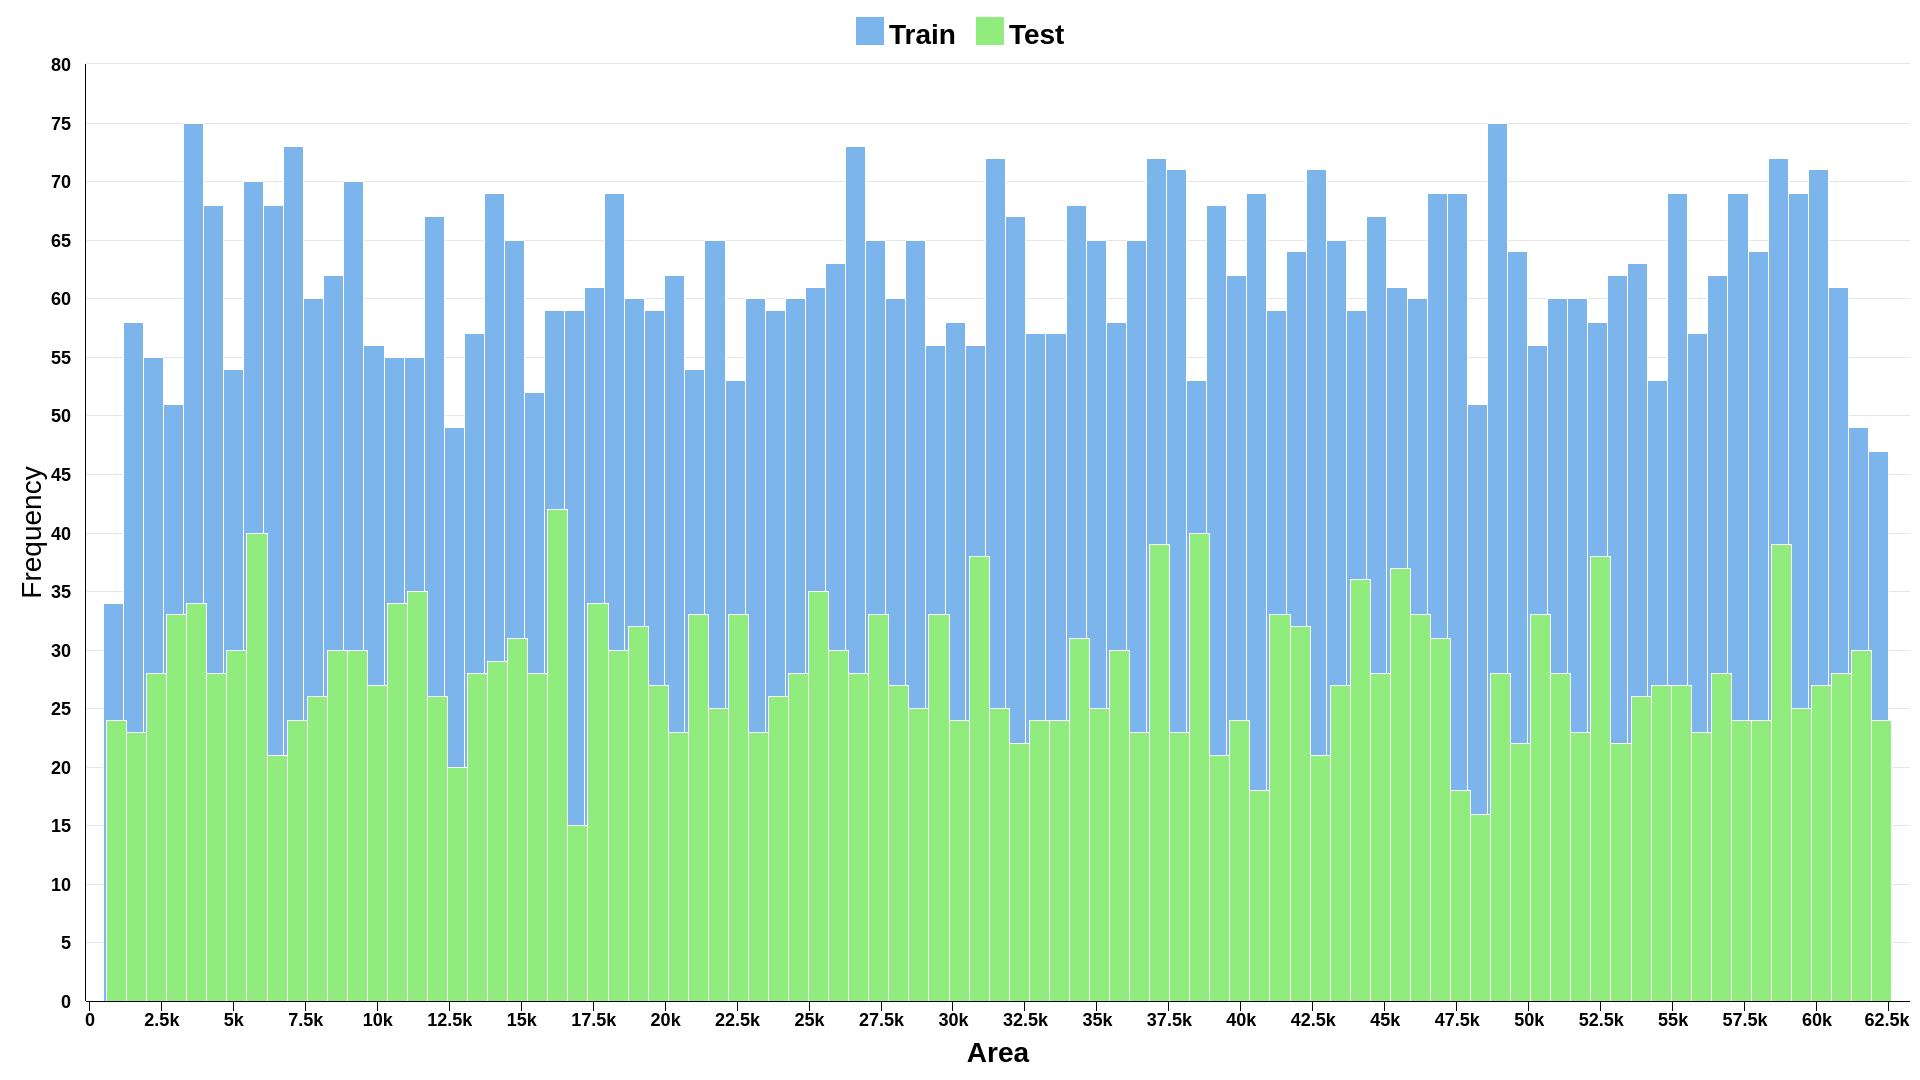
\includegraphics[width=1.0\linewidth]{imgs/Test_5/dataset_5/Partial_Squares_Area_Distribution_Hist.png}
    \caption{Distribuição da Área Visivel (Quadrados Parcial)}
    \label{fig:enter-label}
\end{figure}

\subsection{Treino}

\begin{figure}[H]
    \centering
    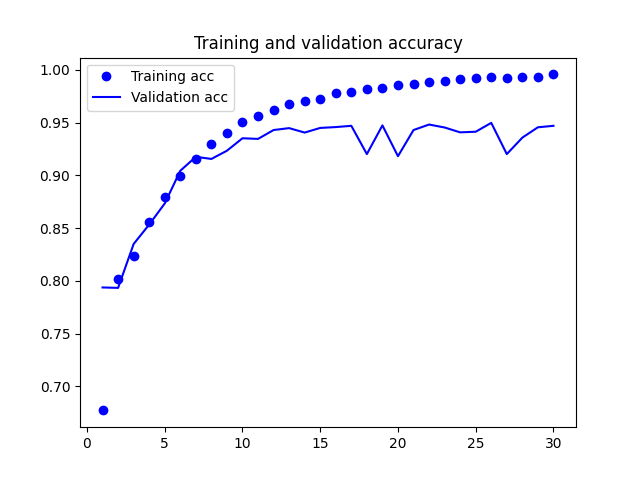
\includegraphics[width=\textwidth]{imgs/Test_5/dataset_5/train_test_acc.png}
    \caption{Acurácia de Validação e de Treino}
    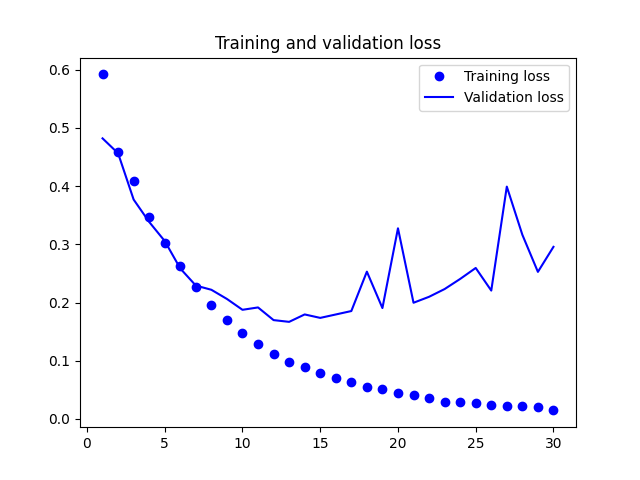
\includegraphics[width=\textwidth]{imgs/Test_5/dataset_5/train_test_loss.png}
    \caption{Perda de Validação e de Treino}
    \label{fig:sub2}
\end{figure}

Foram feitas 30 épocas, alcançando a melhor \texttt{val\_acc} na época 13 de \(94.70\%\).

\subsection{Amostras Mal Classificadas}

No total foram mal classificadas 265 (5.3\% ) imagens, sendo 95 (36\%) delas quadrados normais e as restantes 170 (64\%) quadrados parciais. 

\subsection{Matriz de Confusão}

\begin{table}[H]
\centering
\begin{tabular}{l|c c}
                   & Quadrados & Quadrados Parciais \\
\hline
Quadrados          & 2405         & 170                  \\
Quadrados Parciais & 95           & 2330                  \\
\end{tabular}
\end{table}

\subsection{Metricas de Avaliação}

\begin{table}[H]
\centering
\begin{tabular}{|c|c|c|}
\textit{Acuracy} & \textit{Precision} & \textit{Recall} \\
0.9470 & 0.9470 & 0.9470  \\
\end{tabular}
\end{table}

\subsection{Matriz de Correlação}

\subsection{Conclusão de Teste}
    Bla bla bla


\section{Teste 5.1}
\subsection{Objetivo}
\subsection{Dataset}
\subsection{Treino}
\subsection{Amostras Mal Classificadas}
\subsection{Matriz de Confusão}
\subsection{Metricas de Avaliação}
\subsection{Matriz de Correlação}
\subsection{Conclusão de Teste}
    Bla bla bla


\section{Teste 6}
\subsection{Objetivo}
\subsection{Dataset}
\subsection{Treino}
\subsection{Amostras Mal Classificadas}
\subsection{Matriz de Confusão}
\subsection{Metricas de Avaliação}
\subsection{Matriz de Correlação}
\subsection{Conclusão de Teste}
    Bla bla bla


\section{Teste 6.1}
\subsection{Objetivo}
\subsection{Dataset}
\subsection{Treino}
\subsection{Amostras Mal Classificadas}
\subsection{Matriz de Confusão}
\subsection{Metricas de Avaliação}
\subsection{Matriz de Correlação}
\subsection{Conclusão de Teste}
    Bla bla bla

section{Teste 7}
\subsection{Objetivo}
    O Teste 7 consiste em descobrir quem está mais á direita se o quadrado ou um circulo,estes têm o tamanho igual.
\subsection{Dataset}
O Dataset é composto por 11000 imagens de treino e 5000 de teste. Composto por 2 classes:
\subsection{Treino}
\subsection{Amostras Mal Classificadas}
\subsection{Matriz de Confusão}
\subsection{Metricas de Avaliação}
\subsection{Matriz de Correlação}
\subsection{Conclusão de Teste}
    Bla bla bla

\newpage

\section{Teste 7.1}
\subsection{Objetivo}
    Ver quem está a direita
    Tamanhos iguais
    Com Intesecções
\subsection{Dataset}
O Dataset é composto por 11000 imagens de treino e 5000 de teste. Composto por 2 classes:
\begin{itemize}
        \item Circulo à direita
        \item Quadrado à direita
    \end{itemize}
    Cada imagem tem 2 formas, contendo uma das seguintes combinações:
    \begin{itemize}
        \item Circulo com Circulo
        \item Quadrado com Quadrado
        \item Circulo com Quadrados
    \end{itemize}
    \begin{figure}[H]
        \centering
            
\includegraphics[width=0.25\linewidth]{imgs//Test_7/7_1/dataset/car_5629.png}
            
\includegraphics[width=0.25\linewidth]{imgs//Test_7/7_1/dataset/car_7413.png}
        \caption{Circulo à direita}
        \label{fig:enter-label}
    \end{figure}
    \begin{figure}[H]
        \centering
        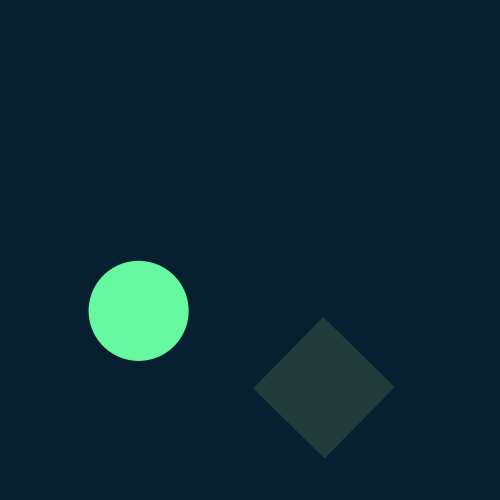
\includegraphics[width=0.25\linewidth]{imgs//Test_7/7_1/dataset/sar_5705.png}
        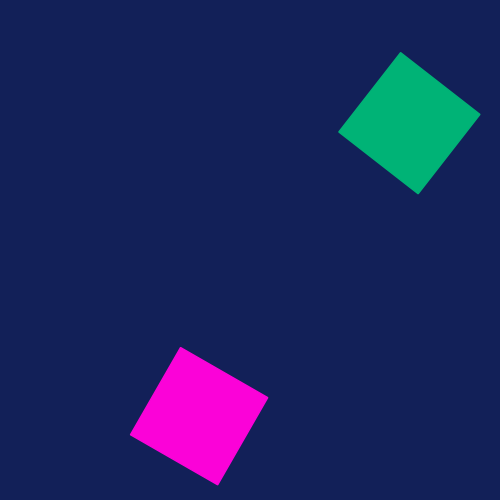
\includegraphics[width=0.25\linewidth]{imgs//Test_7/7_1/dataset/sar_7153.png}
        \caption{Quadrado à direita}
        \label{fig:enter-label}
    \end{figure}
    \begin{figure}[H]
        \centering
        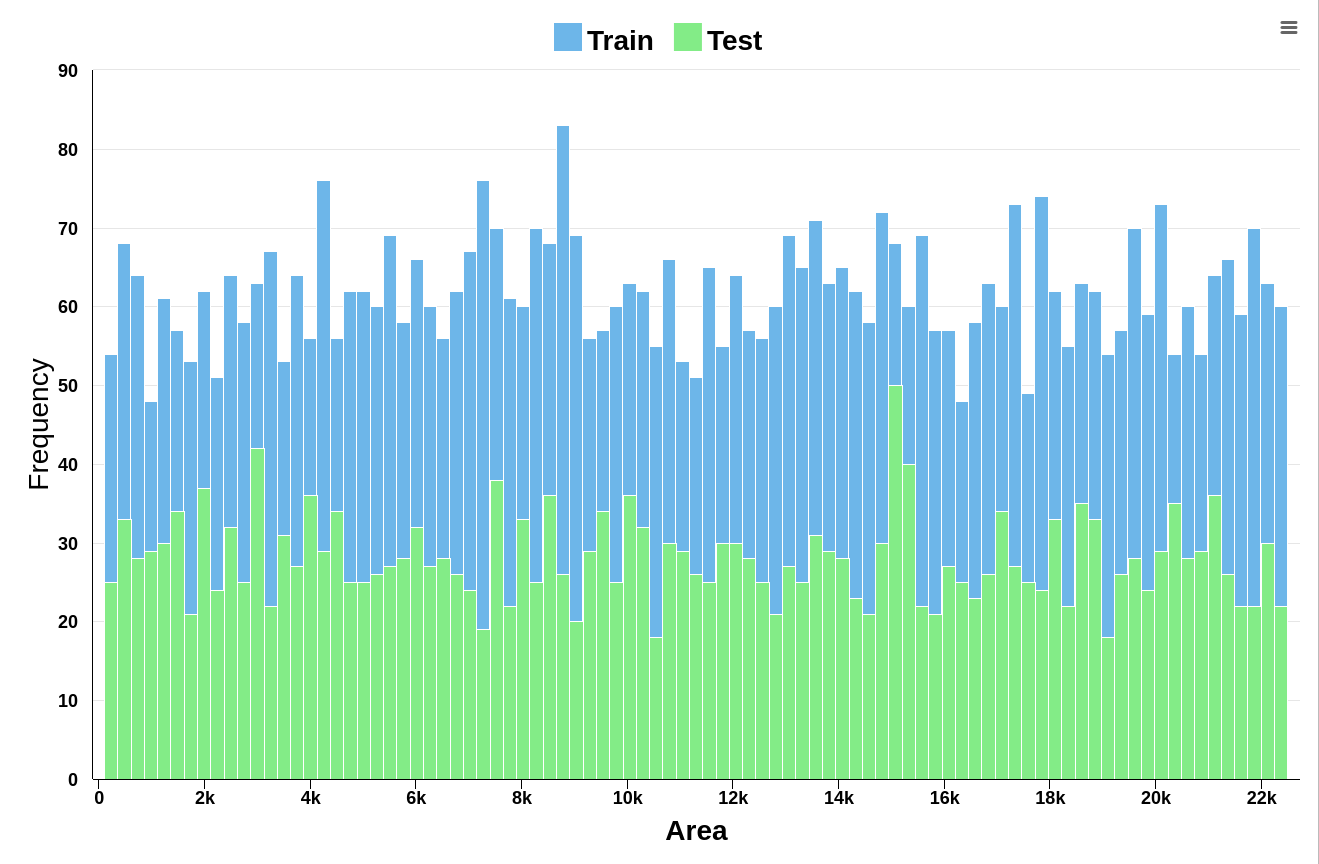
\includegraphics[width=1.0\linewidth]{imgs//Test_7/7_1/dataset/distribution_squares.png}
        \caption{Distribuição da Área (Circulos à direita)}
        \label{fig:enter-label}
    \end{figure}
    \begin{figure}[H]
        \centering
        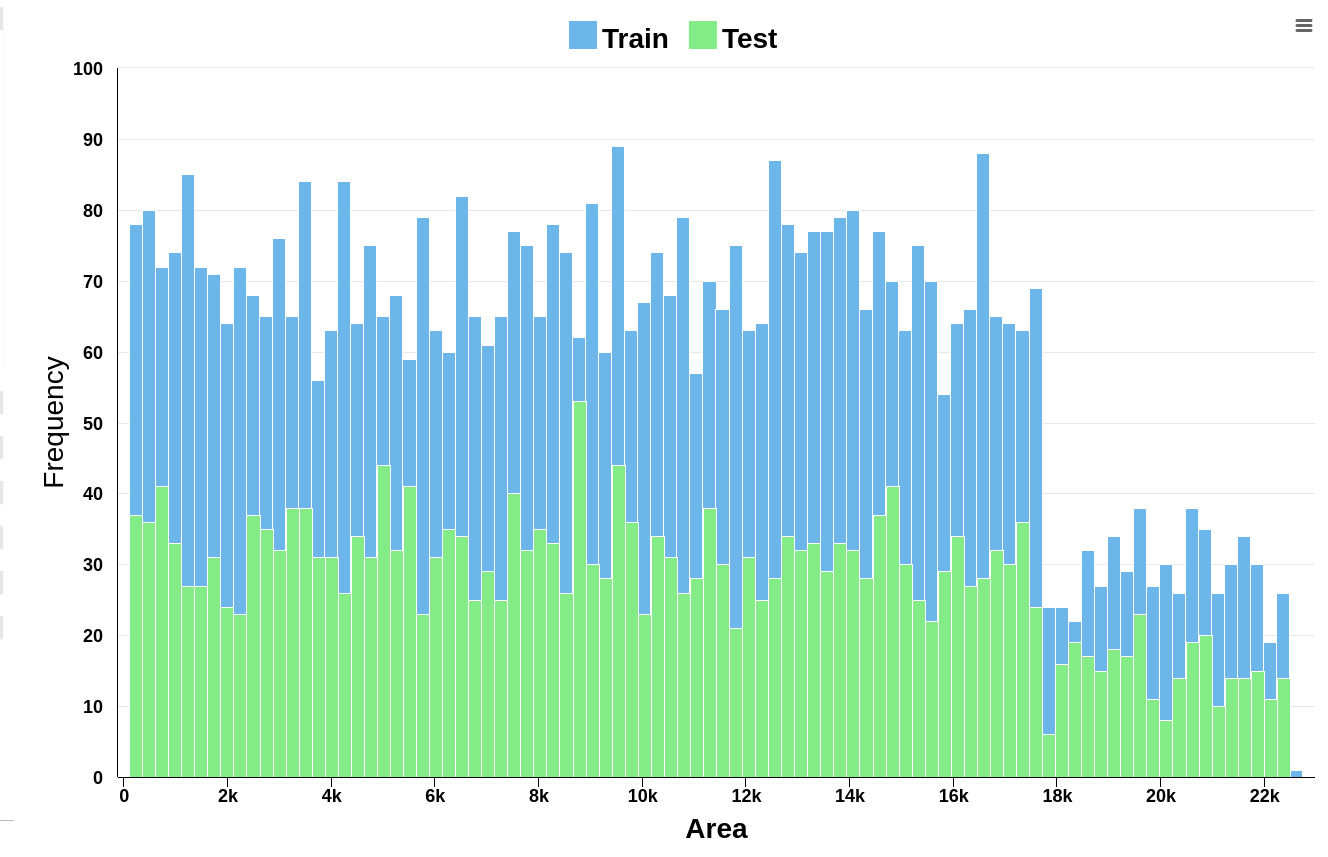
\includegraphics[width=1.0\linewidth]{imgs//Test_7/7_1/dataset/distribution_circles.png}
        \caption{Distribuição da Área (Quadrados à direita)}
        \label{fig:enter-label}
    \end{figure}
\subsection{Treino}
\begin{figure}[H]
    \centering
    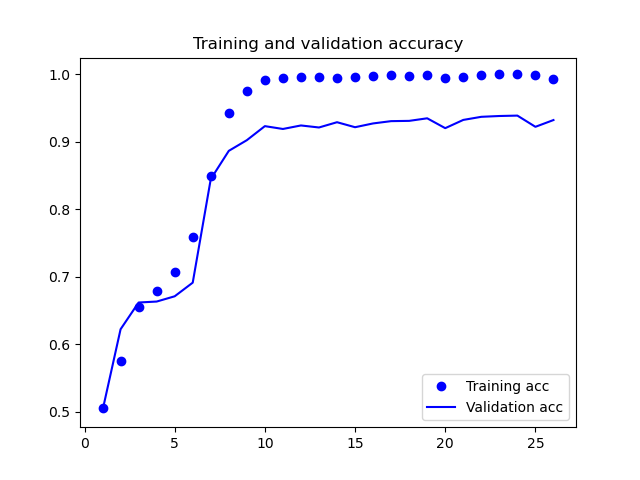
\includegraphics[width=\textwidth]{imgs//Test_7/7_1/train_test_acc.png}
    \caption{Acurácia de Validação e de Treino}
    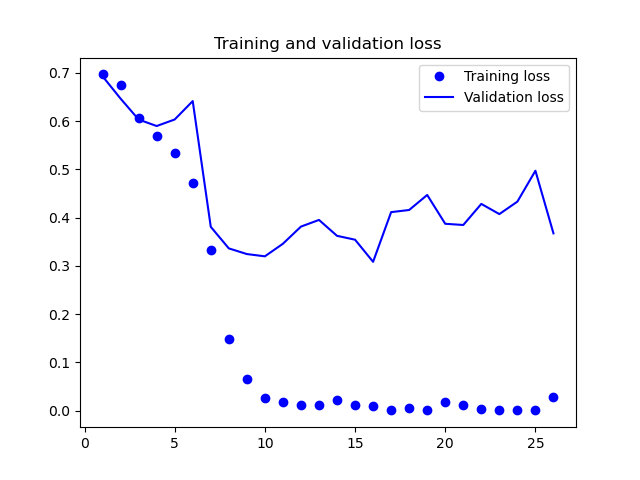
\includegraphics[width=\textwidth]{imgs//Test_7/7_1/train_test_loss.png}
    \caption{Perda de Validação e de Treino}
    \label{fig:sub2}
    Com as 26 épocas realizadas, conseguimos uma val acc de 0.9024, sendo que a melhor loss foi atingida na época 10.
\end{figure}
\subsection{Amostras Mal Classificadas}
No total foram mal classificadas 339 (13.74\% ) imagens de teste sendo:
    - 65 imagens com circulo à direita com um quadrado à esquerda
    - 44 imagens com circulo à direita e à esquerda
    - 86 imagens com quadrado à direita e com um circulo à esquerda 
    - 144 imagens com quadrado à direita e à esquerda
    

\subsection{Matriz de Confusão}

\begin{table}[H]
\centering
\begin{tabular}{l|c c}
                & Circulo à Direita & Quadrado à Direita \\ 
\hline
Circulo à Direita         & 2391         & 109                  \\
Quadrado à Direita        & 230         & 2270                 \\

\end{tabular}
\end{table}

\subsection{Metricas de Avaliação}
\subsection{Matriz de Correlação}
\subsection{Conclusão de Teste}
    Bla bla bla

\newpage

\section{Teste 7.2}
\subsection{Objetivo}
    Este teste é bastante semelhante ao teste 7, ao seja o objetivo é identificar entre um quadrado ou circulo, qual o que está mais á direita na imagem. Neste caso os tamanhos das formas podem ser diferente um do outro
\subsection{Dataset}
O Dataset é composto por 11000 imagens de treino e 5000 de teste. Composto por 2 classes:
    \begin{itemize}
        \item Circulo à direita
        \item Quadrado à direita
    \end{itemize}
    Cada imagem tem 2 formas, contendo uma das seguintes combinações:
    \begin{itemize}
        \item Circulo com Circulo
        \item Quadrado com Quadrado
        \item Circulo com Quadrados
    \end{itemize}
    \begin{figure}[H]
        \centering
            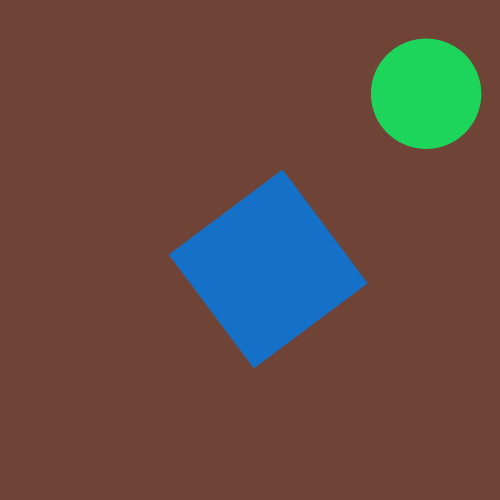
\includegraphics[width=0.25\linewidth]{imgs/Test_7/7_2/dataset/car_1.png}
            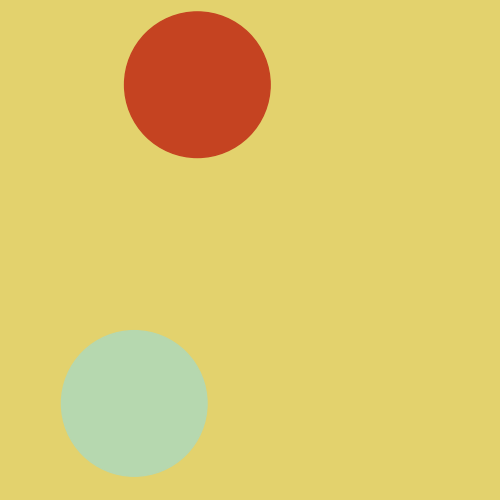
\includegraphics[width=0.25\linewidth]{imgs/Test_7/7_2/dataset/car_3116.png}
        \caption{Circulo à direita}
        \label{fig:enter-label}
    \end{figure}
    \begin{figure}[H]
        \centering
        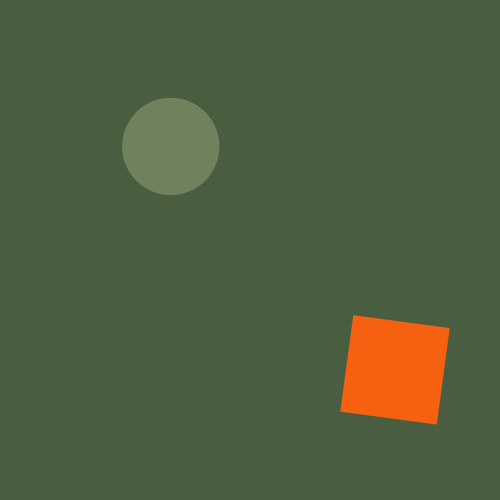
\includegraphics[width=0.25\linewidth]{imgs/Test_7/7_2/dataset/sar_9.png}
        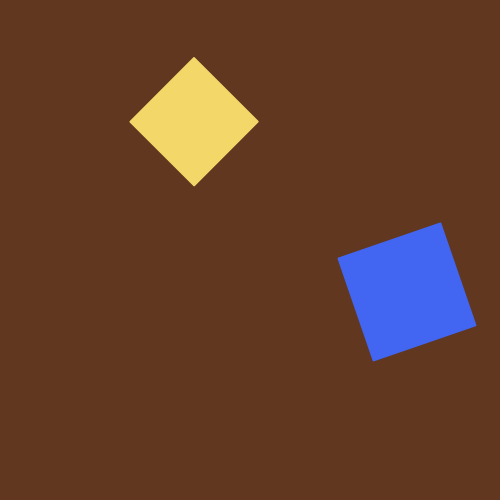
\includegraphics[width=0.25\linewidth]{imgs/Test_7/7_2/dataset/sar_3873.png}
        \caption{Quadrado à direita}
        \label{fig:enter-label}
    \end{figure}
    \begin{figure}[H]
        \centering
        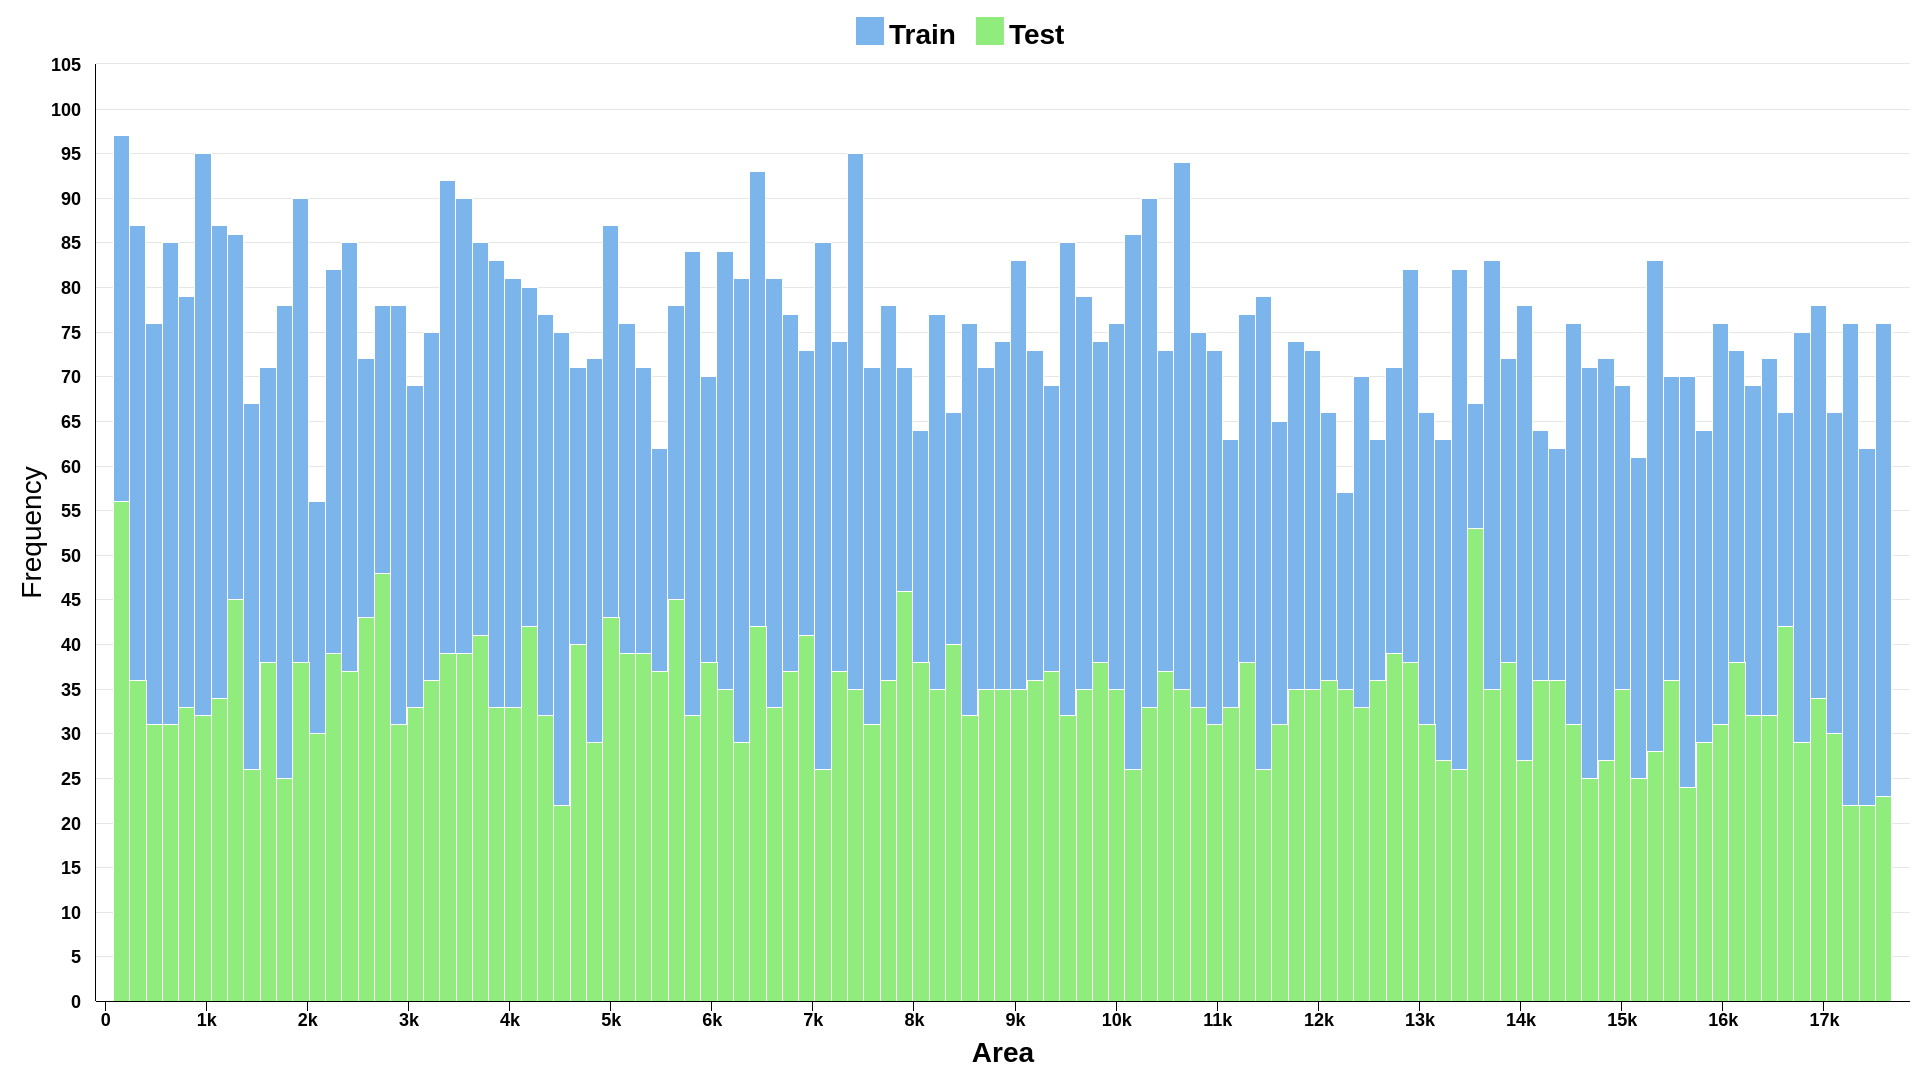
\includegraphics[width=1.0\linewidth]{imgs/Test_7/7_2/dataset/car_ci_distribution_hist.png}
        \caption{Distribuição da Área (Circulos à direita)}
        \label{fig:enter-label}
    \end{figure}
    \begin{figure}[H]
        \centering
        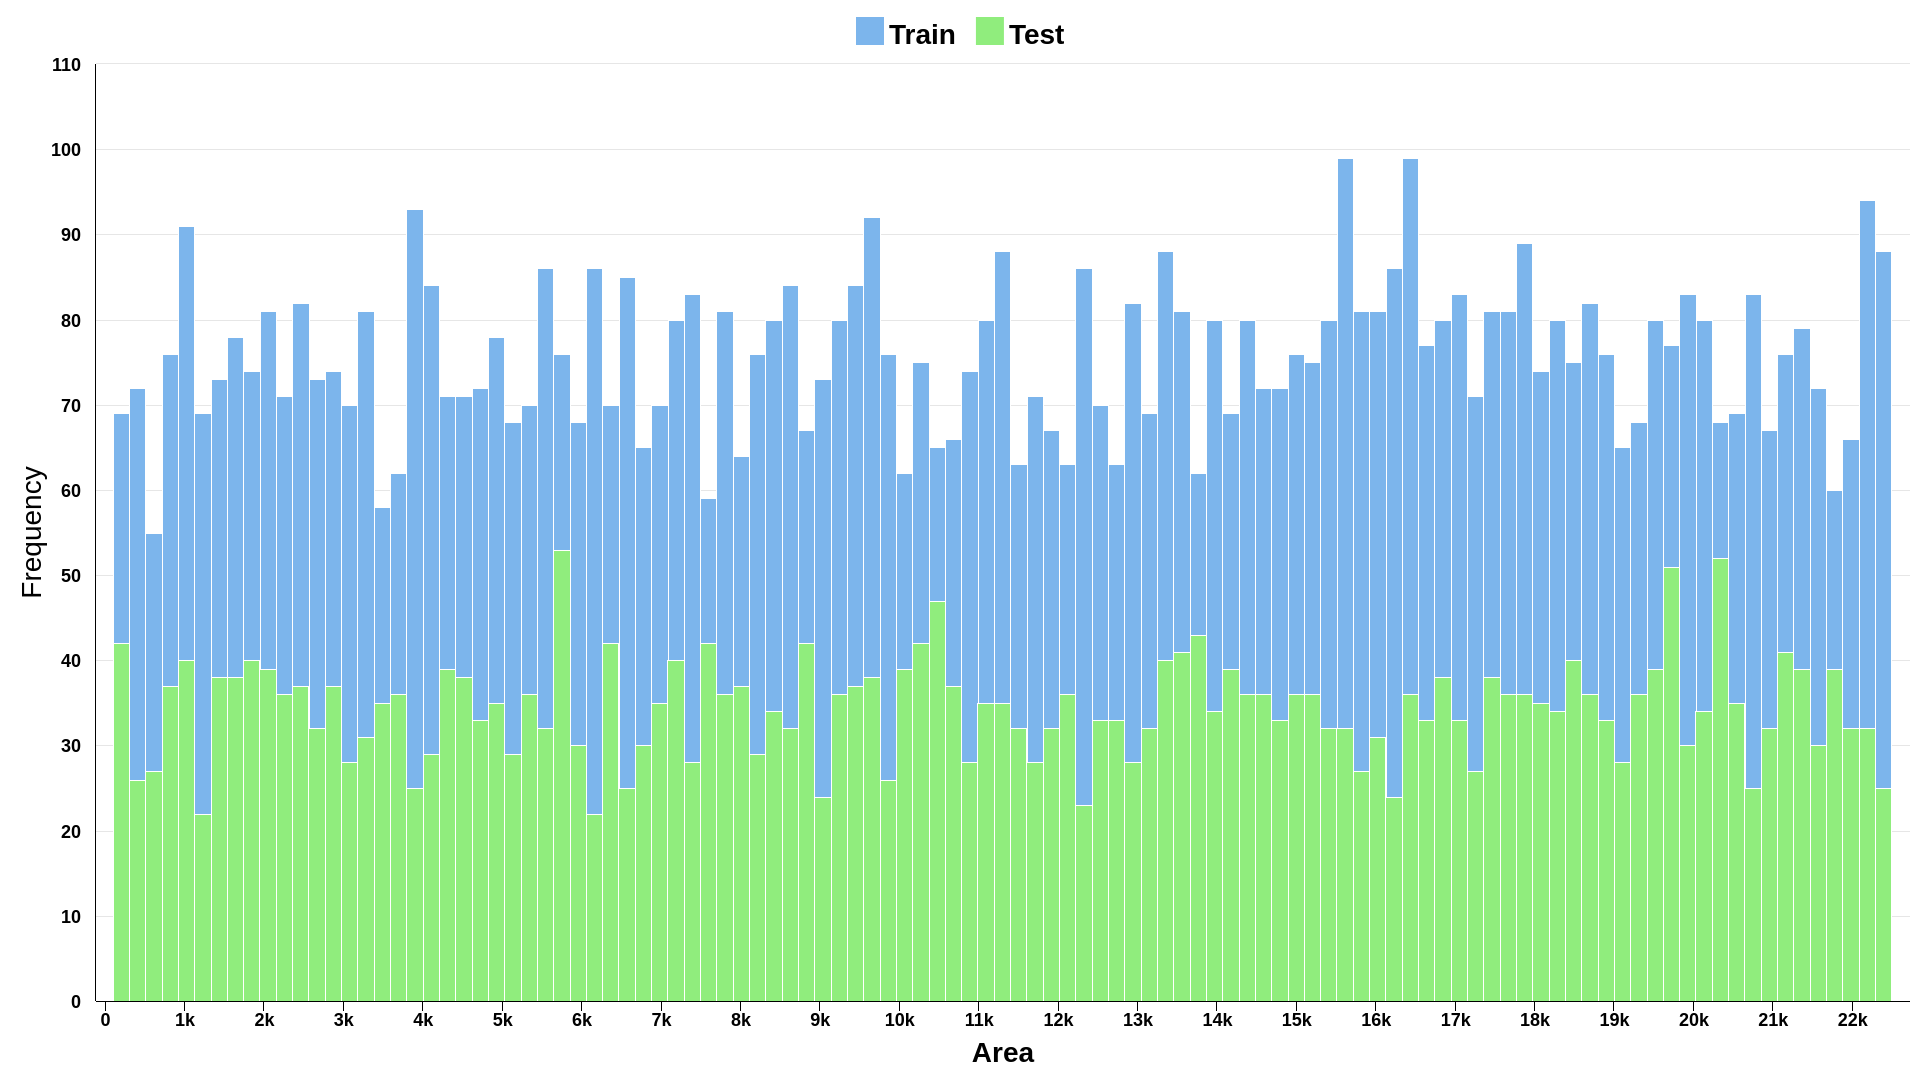
\includegraphics[width=1.0\linewidth]{imgs/Test_7/7_2/dataset/sar_sq_distribution_hist.png}
        \caption{Distribuição da Área (Quadrados à direita)}
        \label{fig:enter-label}
    \end{figure}
\subsection{Treino}
\begin{figure}[H]
    \centering
    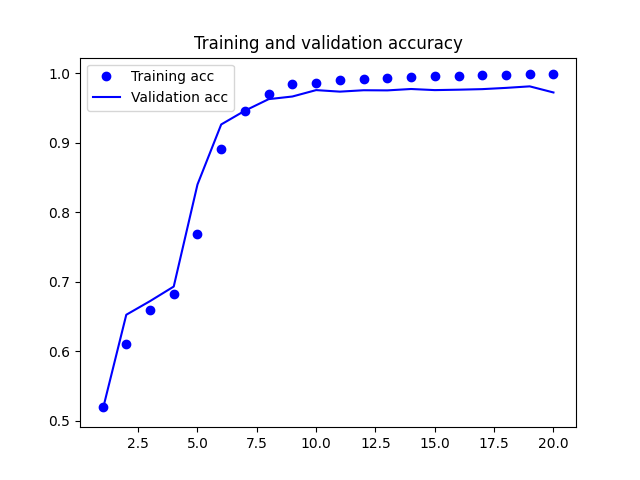
\includegraphics[width=\textwidth]{imgs/Test_7/7_2/train_test_acc.png}
    \caption{Acurácia de Validação e de Treino}
    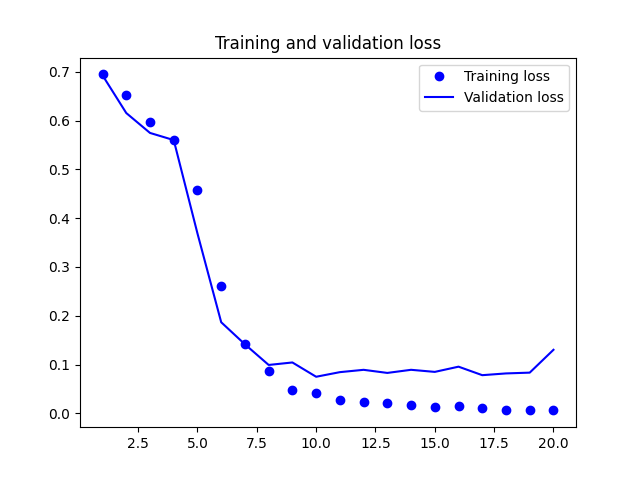
\includegraphics[width=\textwidth]{imgs/Test_7/7_2/train_test_loss.png}
    \caption{Perda de Validação e de Treino}
    \label{fig:sub2}
    Com as 20 épocas realizadas, conseguimos uma val acc de 0.9720, sendo que a melhor loss foi atingida na época 10.
\end{figure}

\subsection{Amostras Mal Classificadas}

No total foram mal classificadas 140 (2.8\% ) imagens sendo:
 \begin{itemize}
    \item 0 imagens com circulo à direita com um quadrado à esquerda
    \item 13 imagens com circulo à direita e à esquerda
    \item 45 imagens com quadrado à direita e com um circulo à esquerda 
    \item 52 imagens com quadrado à direita e à esquerda
\end{itemize}
    

\subsection{Matriz de Confusão}

\begin{table}[H]
\centering
\begin{tabular}{l|c c}
                & Circulo à Direita & Quadrado à Direita \\
\hline
Circulo à Direita         & 2406         & 97                  \\
Quadrado à Direita        & 43         & 2457                 \\

\end{tabular}
\end{table}

\subsection{Análise}
\begin{figure}[H]
    \centering
    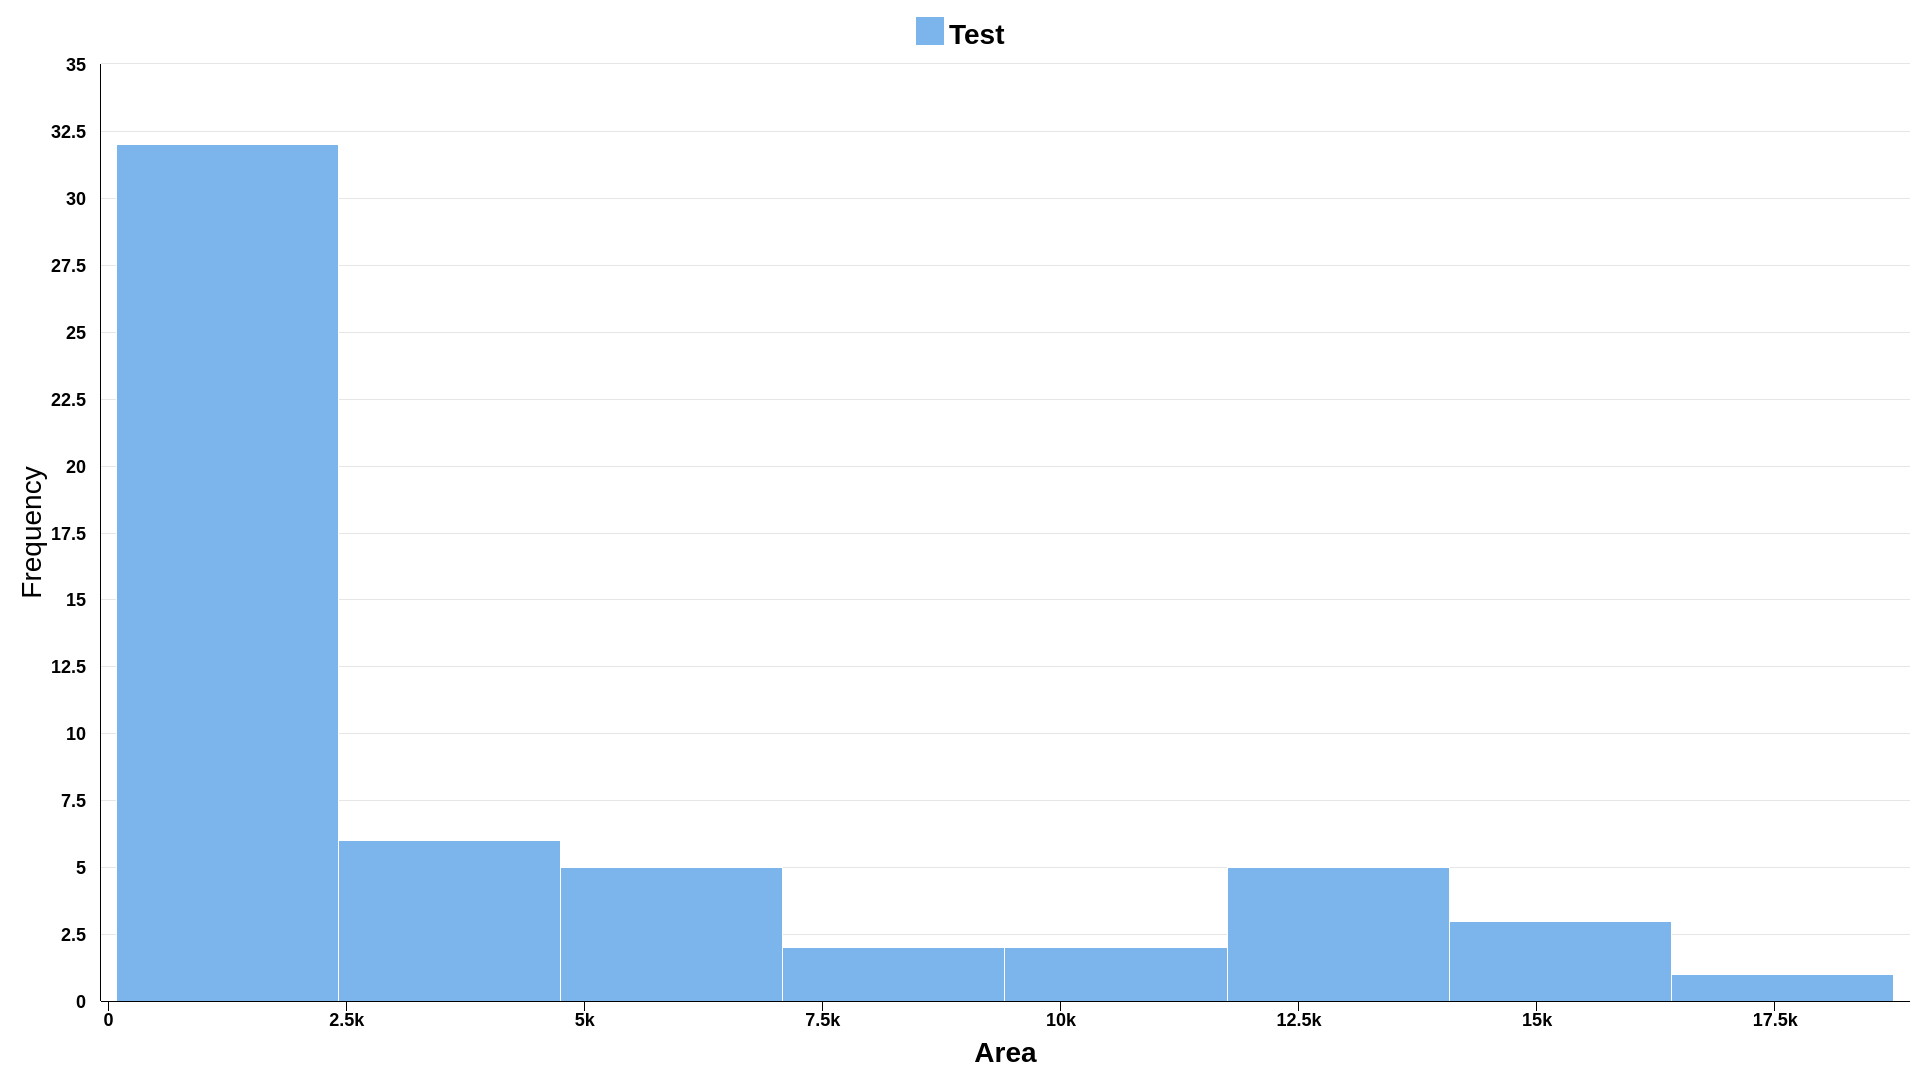
\includegraphics[width=\textwidth]{imgs/Test_7/7_2/failed/car_ci_failed_area_hist.png}
    \caption{Distribuição da Área dos Circulos à direita }
    \label{fig:sub2}
\end{figure}

\begin{figure}[H]
    \centering
    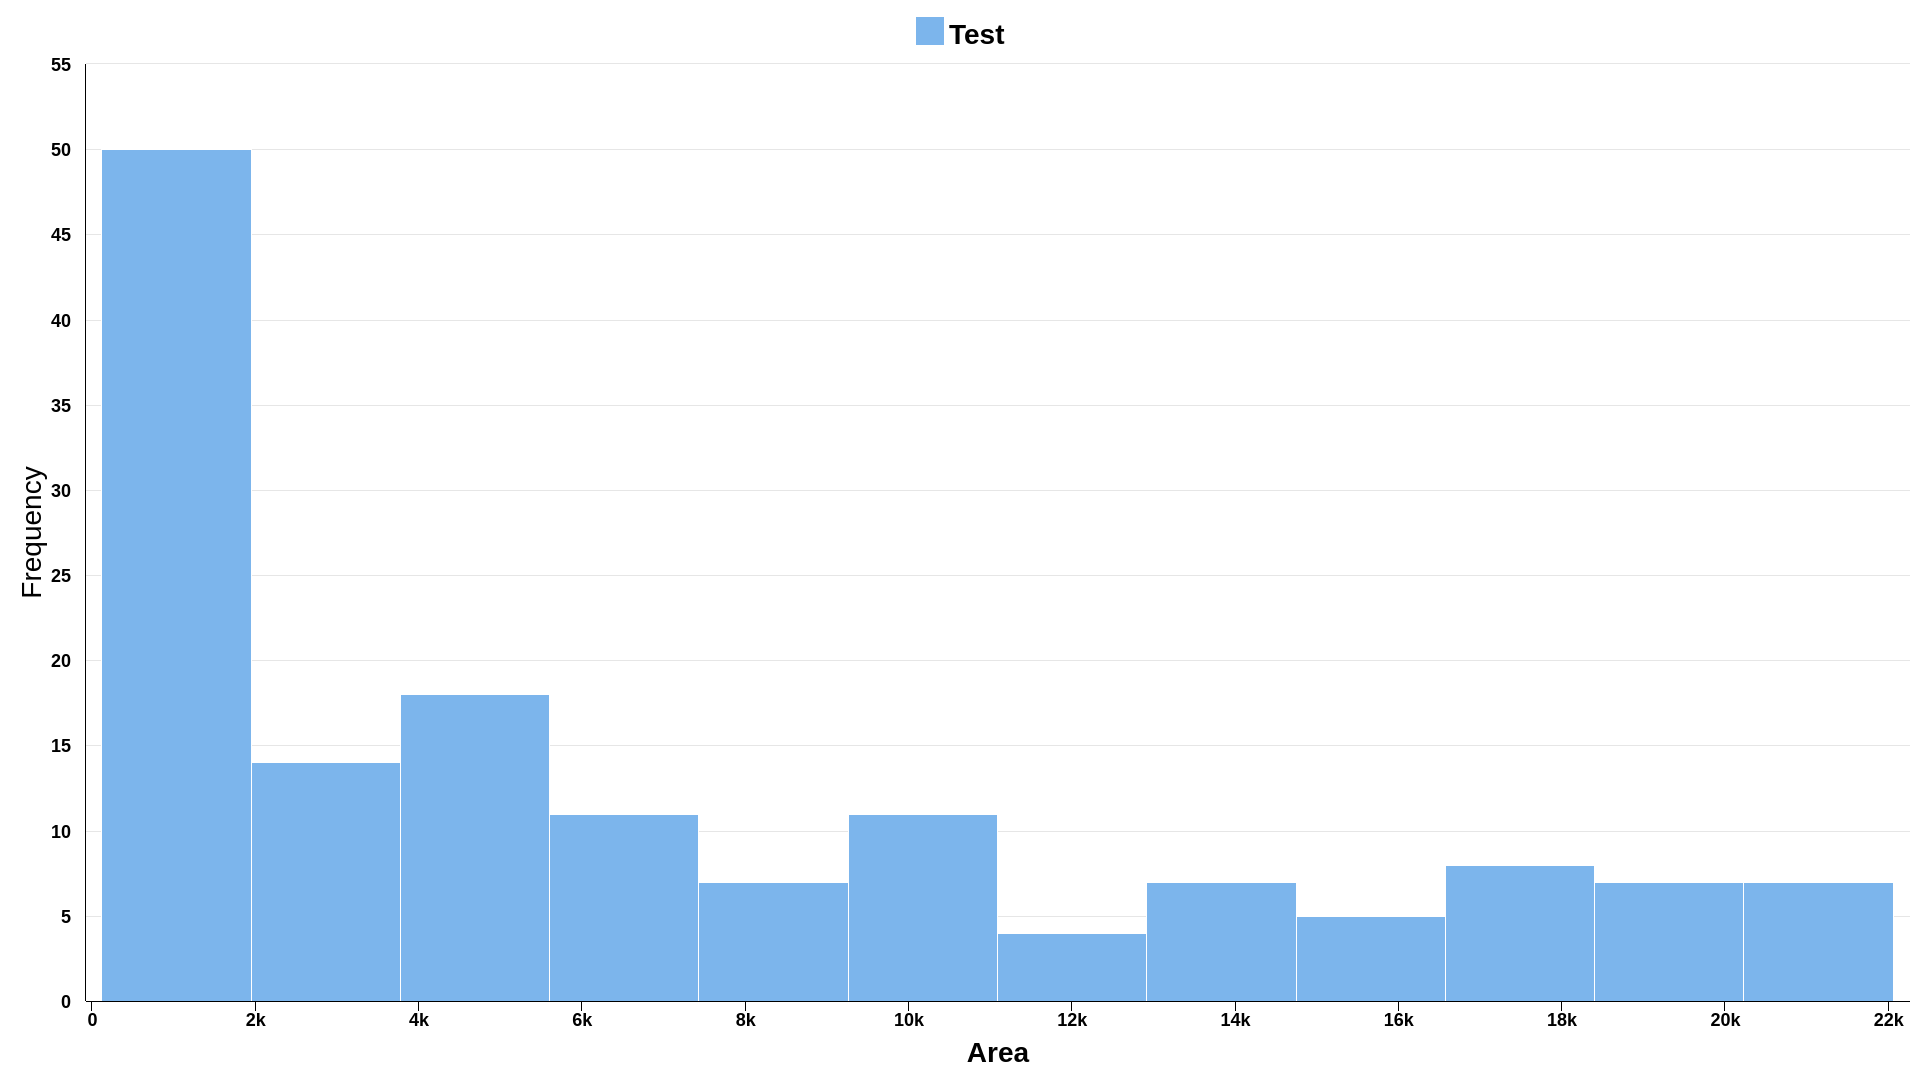
\includegraphics[width=\textwidth]{imgs/Test_7/7_2/failed/sar_sq_failed_area_hist.png}
    \caption{Distribuição da Área dos Quadrados à direita }
    \label{fig:sub2}
\end{figure}

\begin{figure}[H]
    \centering
    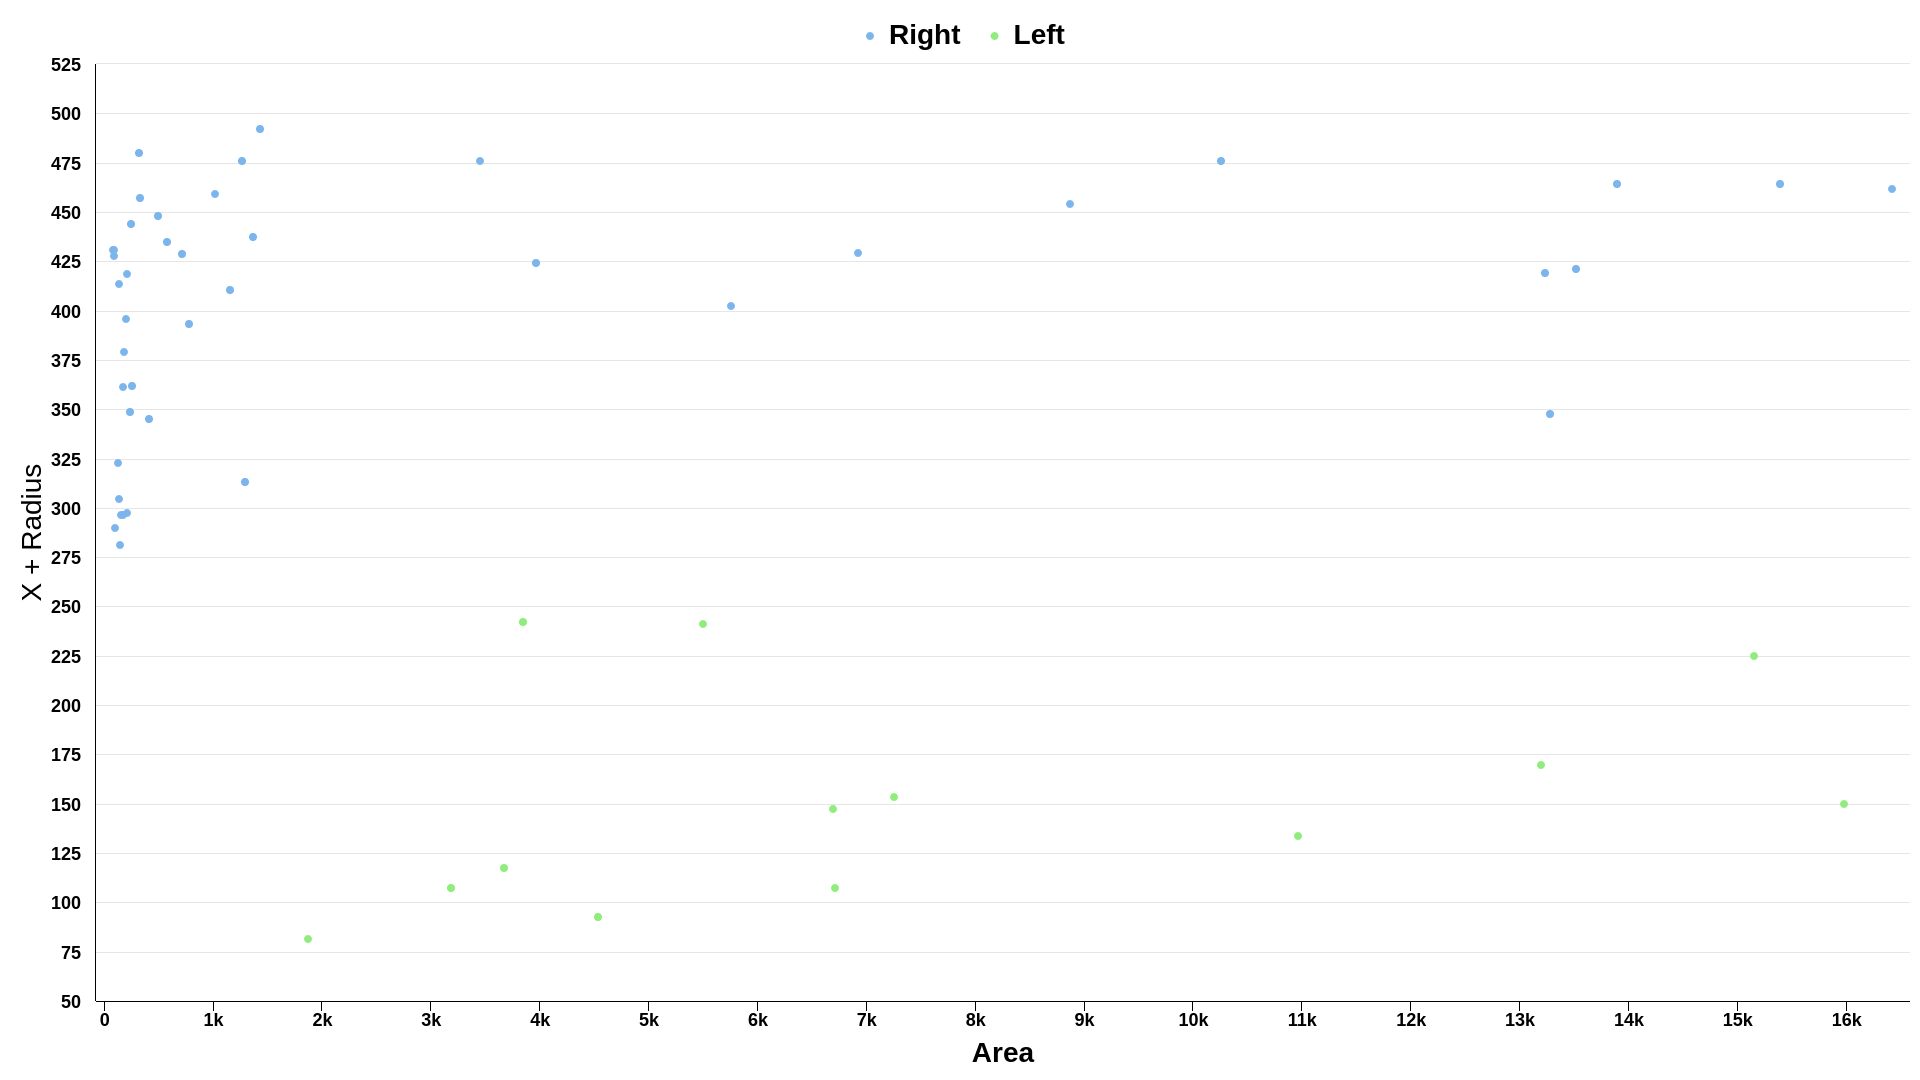
\includegraphics[width=\textwidth]{imgs/Test_7/7_2/failed/car_ci_failed_right_left_scatter.png}
    \caption{Scatter dos circulos, em imagens de circulos à direita}
    \label{fig:sub2}
\end{figure}

\begin{figure}[H]
    \centering
    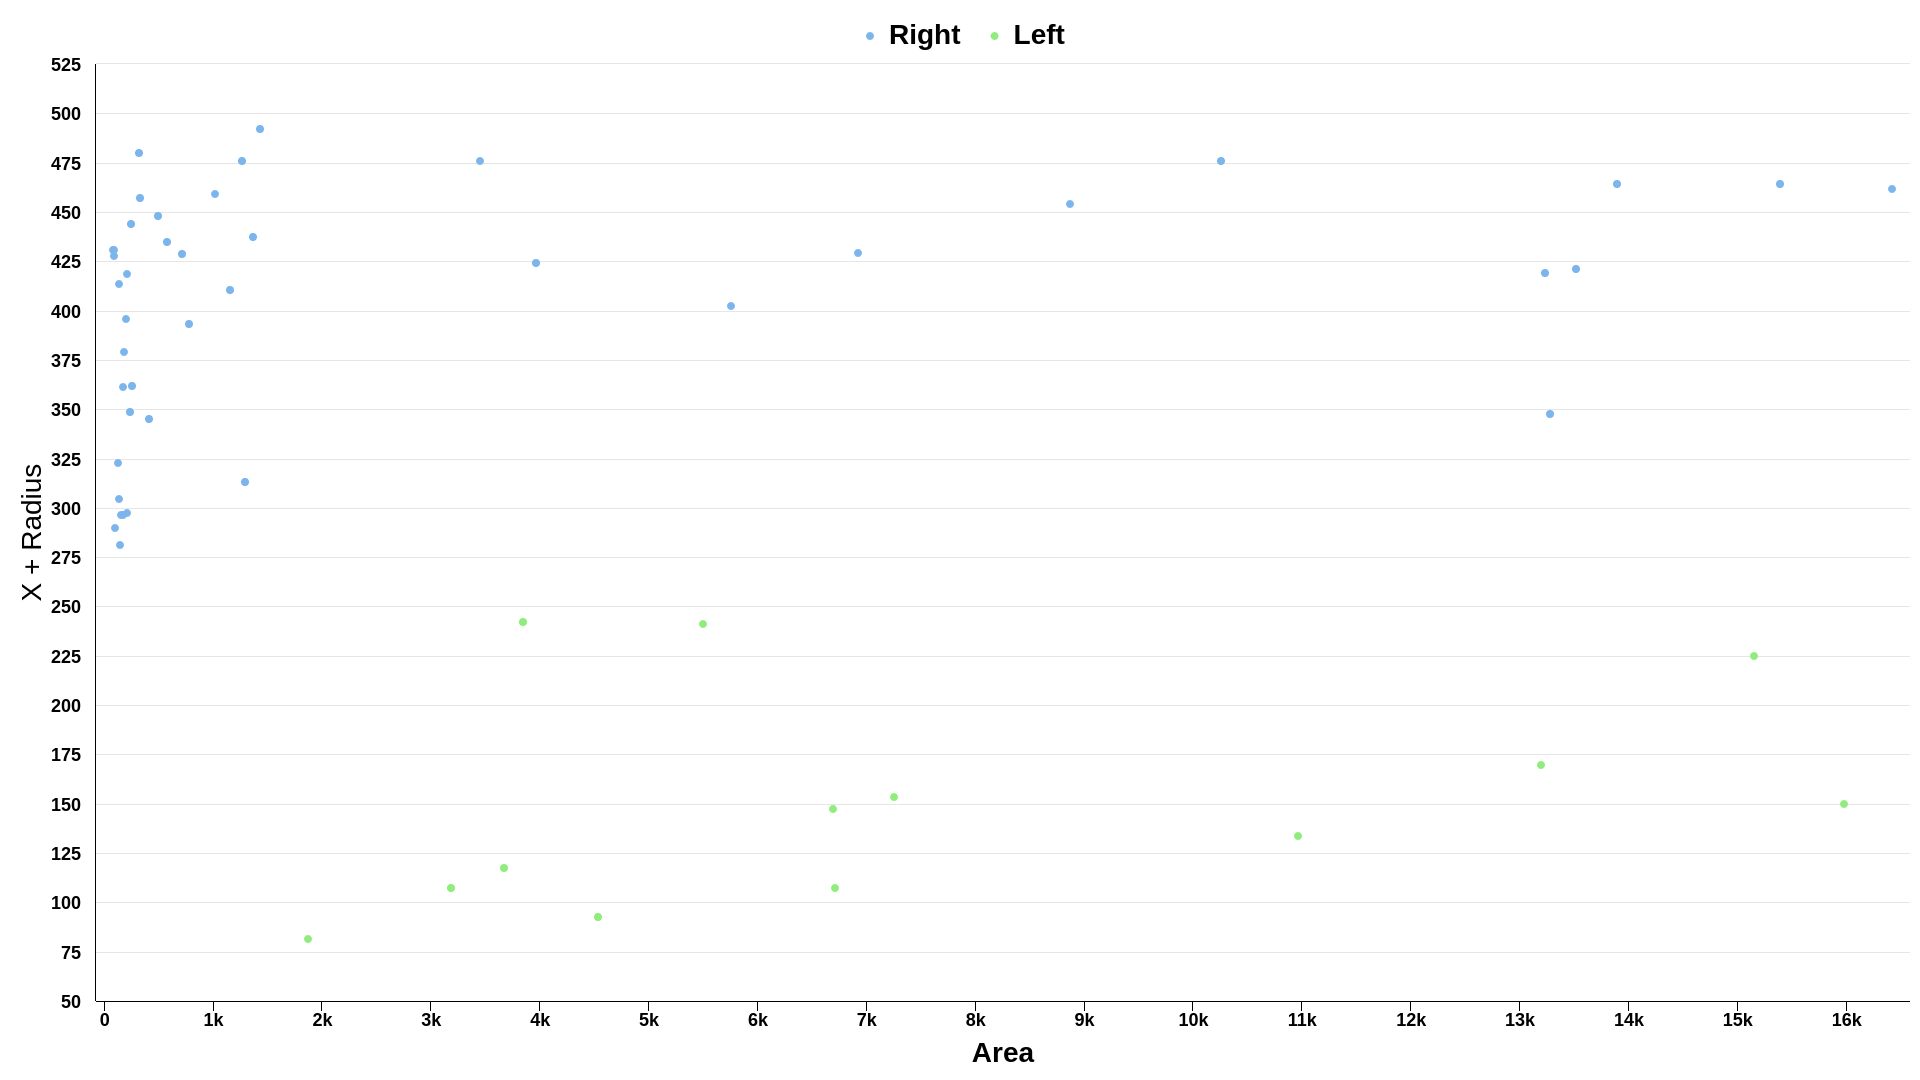
\includegraphics[width=\textwidth]{imgs/Test_7/7_2/failed/car_ci_failed_right_left_scatter.png}
    \caption{Scatter dos quadrados, em imagens de quadrados à direita}
    \label{fig:sub2}
\end{figure}

Como podemos ver partir dos histogramas, o que causa o modelo ao engano é quando numa imagem está presente circulos ou quadrados muito pequenos. Um pormenor que é possivel observar, principalmente no scatter dos quadrados, é que o que está á esquerda não influencia muito devido ao tamanho, o tamanho só influencia caso esse esteja à direita


\section{Teste 7.3}
\subsection{Objetivo}
    Ver quem está a direita
    Tamanhos diferentes
    Com Intersecções


\section{Teste 8-ALT}
\subsection{Objetivo}
       Circlos com Circlos
       Ver Porpoção
    
    

\section{Teste 8}
\subsection{Objetivo}

\subsection{Dataset}
    O Dataset é composto por 5500 imagens de treino e 2500 de teste. Composto por apenas imagens com 1 circulo.
    Este dataset foi tambem utilizado no teste 5_1.
    
   
        \begin{figure}[H]
        \centering
        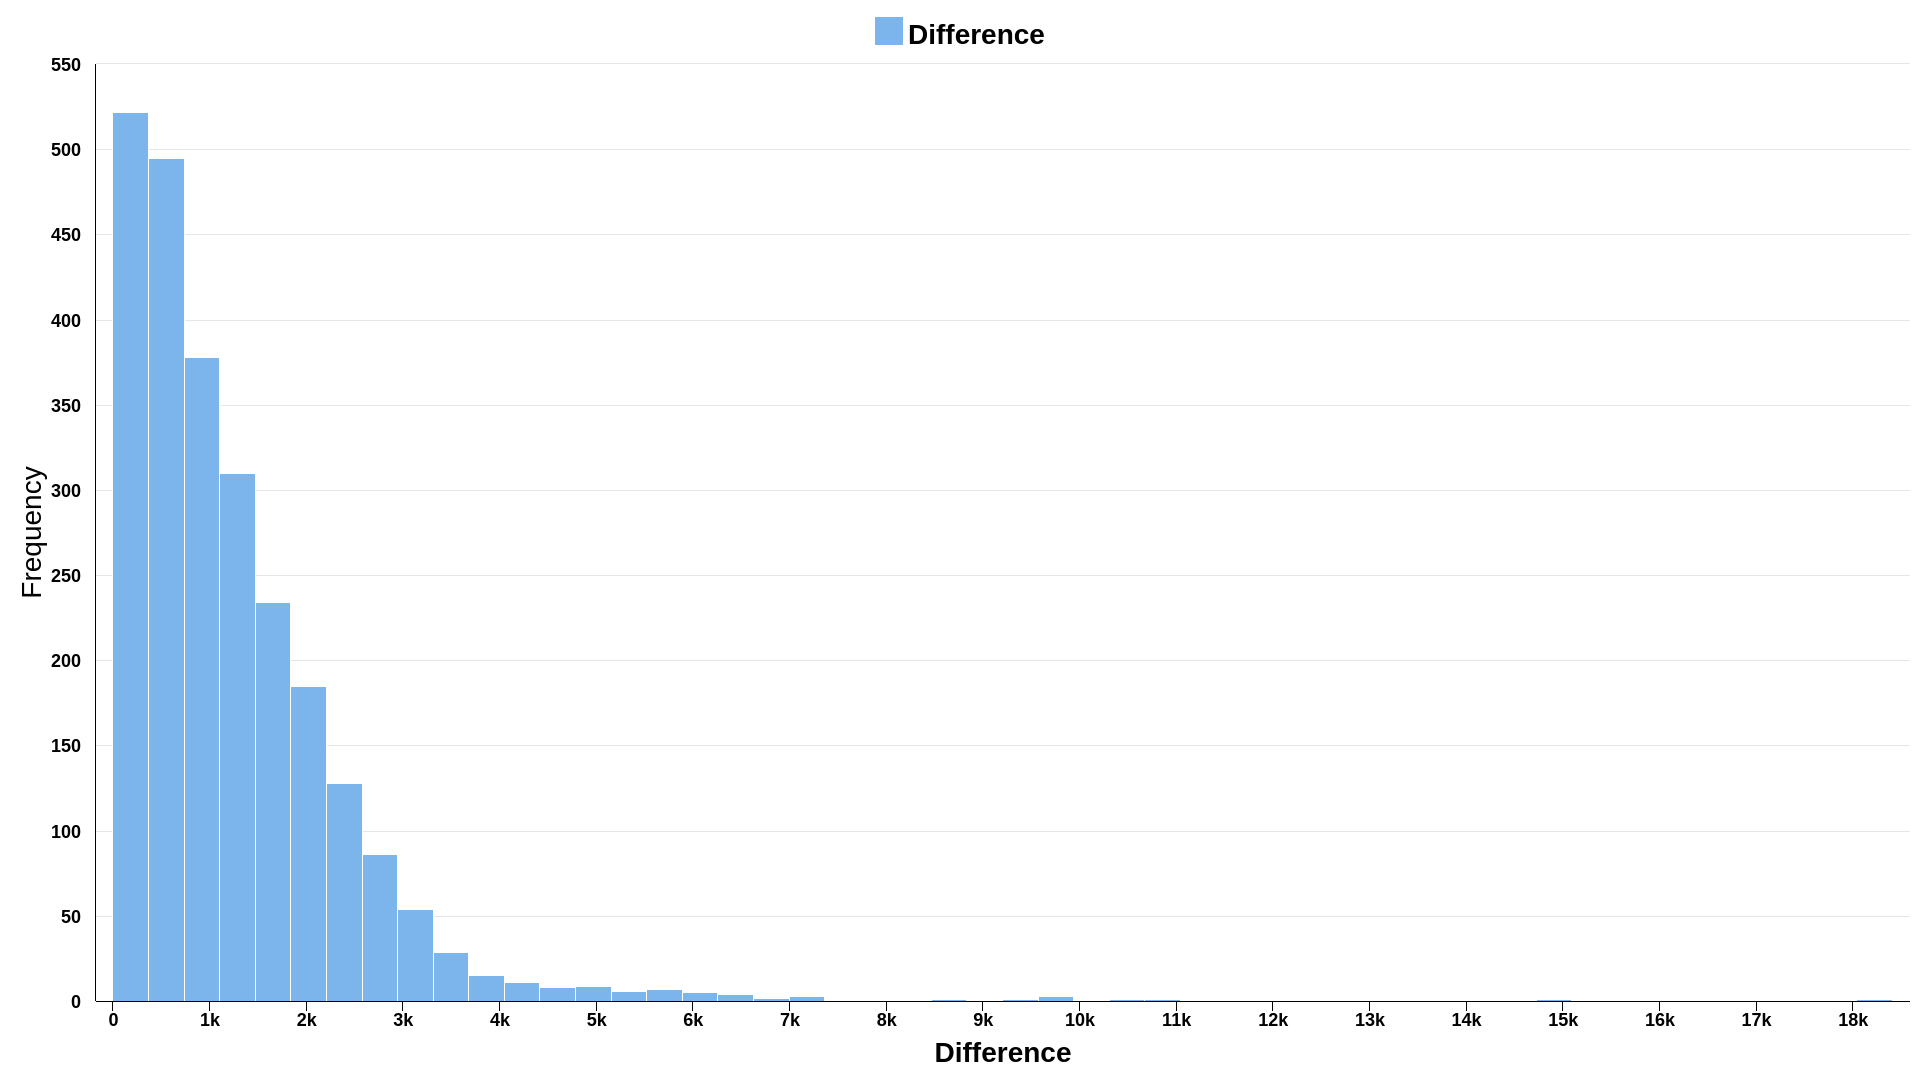
\includegraphics[width=1.0\linewidth]{imgs/Test_8/area_diference_hist.png}

        \label{fig:enter-label}
    \end{figure}
    
       
        \begin{figure}[H]
        \centering
        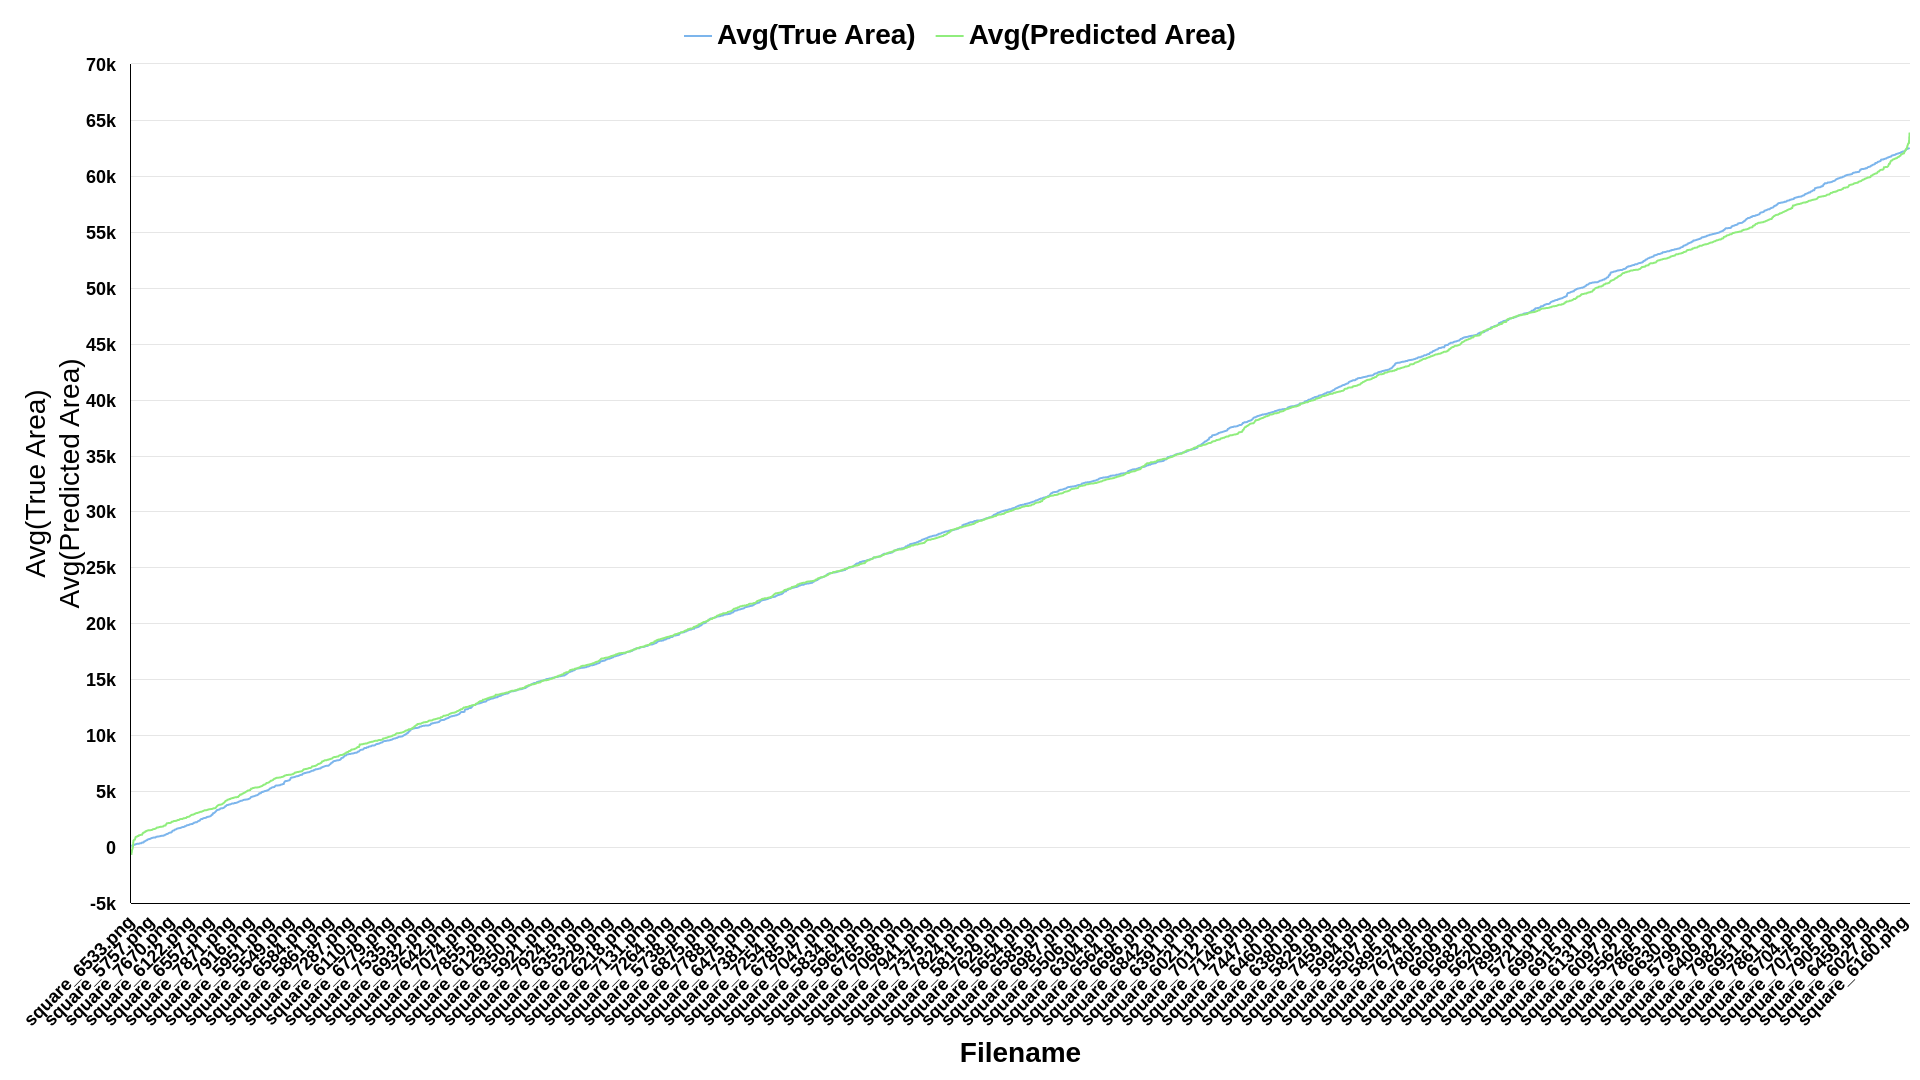
\includegraphics[width=1.0\linewidth]{imgs/Test_8/area_predict_true_line.png}
        \label{fig:enter-label}
    \end{figure}
    
       
        \begin{figure}[H]
        \centering
        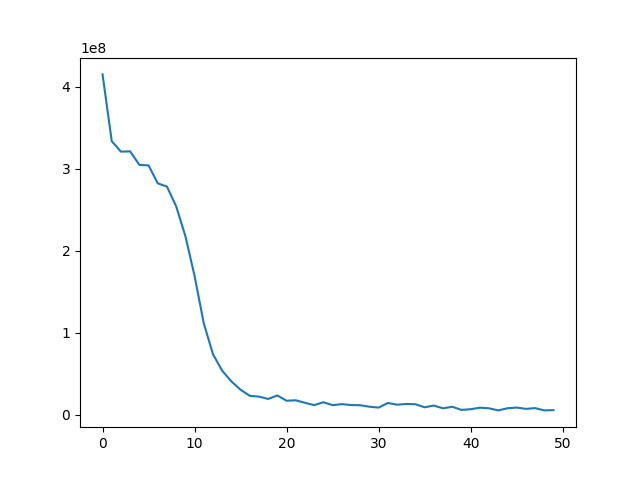
\includegraphics[width=1.0\linewidth]{imgs/Test_8/loss.png}
 
        \label{fig:enter-label}
    \end{figure}
    
       
        \begin{figure}[H]
        \centering
        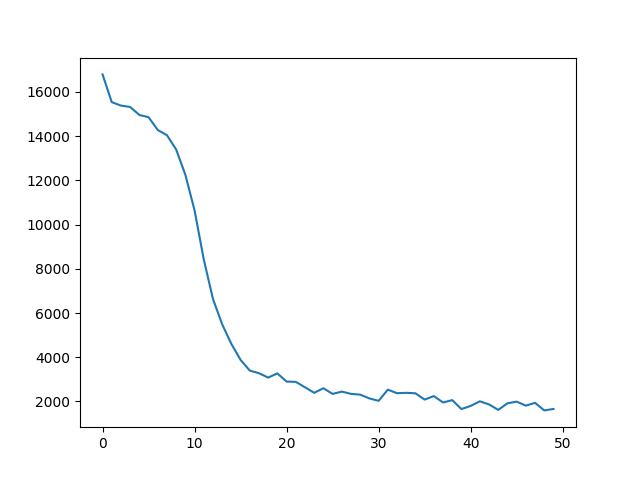
\includegraphics[width=1.0\linewidth]{imgs/Test_8/mae.png}
  
        \label{fig:enter-label}
    \end{figure}
    
    

\section{Teste 9}
\subsection{Objetivo}
    Classificar Imagens com quadrados, circulos e vazios. Ao seja, um problema de classificação não binário.
\subsection{Dataset}
    O Dataset é composto por 10998 imagens de treino e 4998 de teste. Composto por 3 classes: 
    \begin{itemize}
        \item Circulos 
        \item Quadrados
        \item Vazios
    \end{itemize}
    \begin{figure}[H]
        \centering
        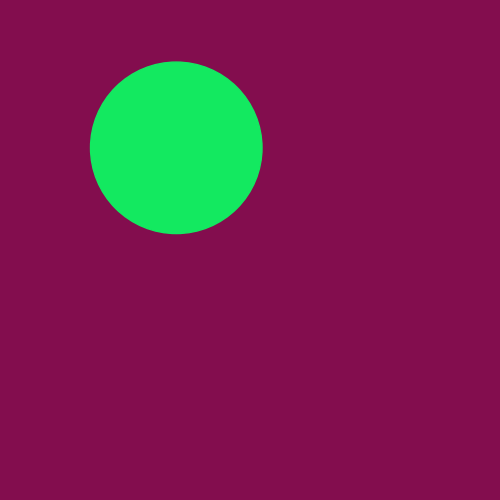
\includegraphics[width=0.25\linewidth]{imgs/Test_9/dataset_9/circles_4.png}
        
\includegraphics[width=0.25\linewidth]{imgs/Test_9/dataset_9/squares_4.png}
        
\includegraphics[width=0.25\linewidth]{imgs/Test_9/dataset_9/nones_3.png}
        \caption{Circlos, Quadrados e Vazios}
        \label{fig:enter-label}
    \end{figure}
    \begin{figure}[H]
        \centering
        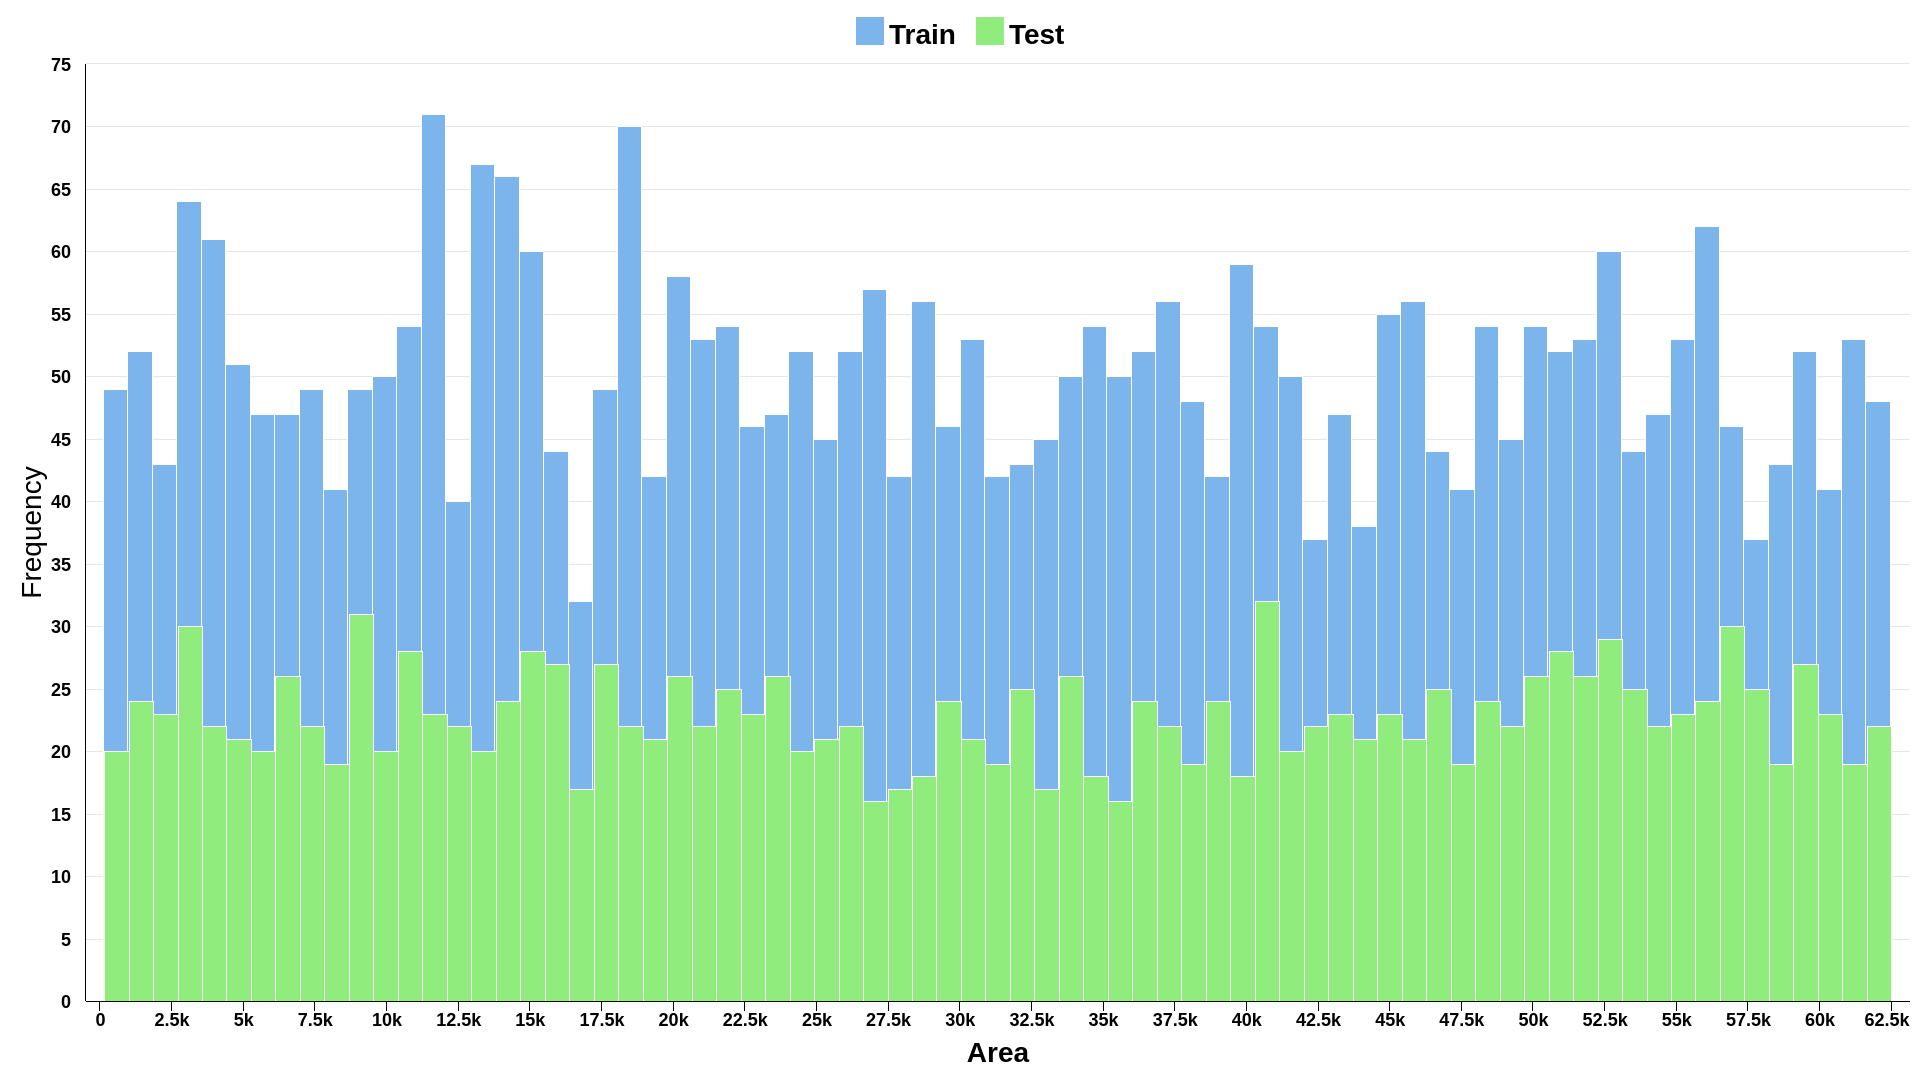
\includegraphics[width=1.0\linewidth]{imgs/Test_9/dataset_9/Squares_Area_Distribution_Hist.png}
        \caption{Distribuição da Área (Quadrados)}
        \label{fig:enter-label}
    \end{figure}
    \begin{figure}[H]
        \centering
        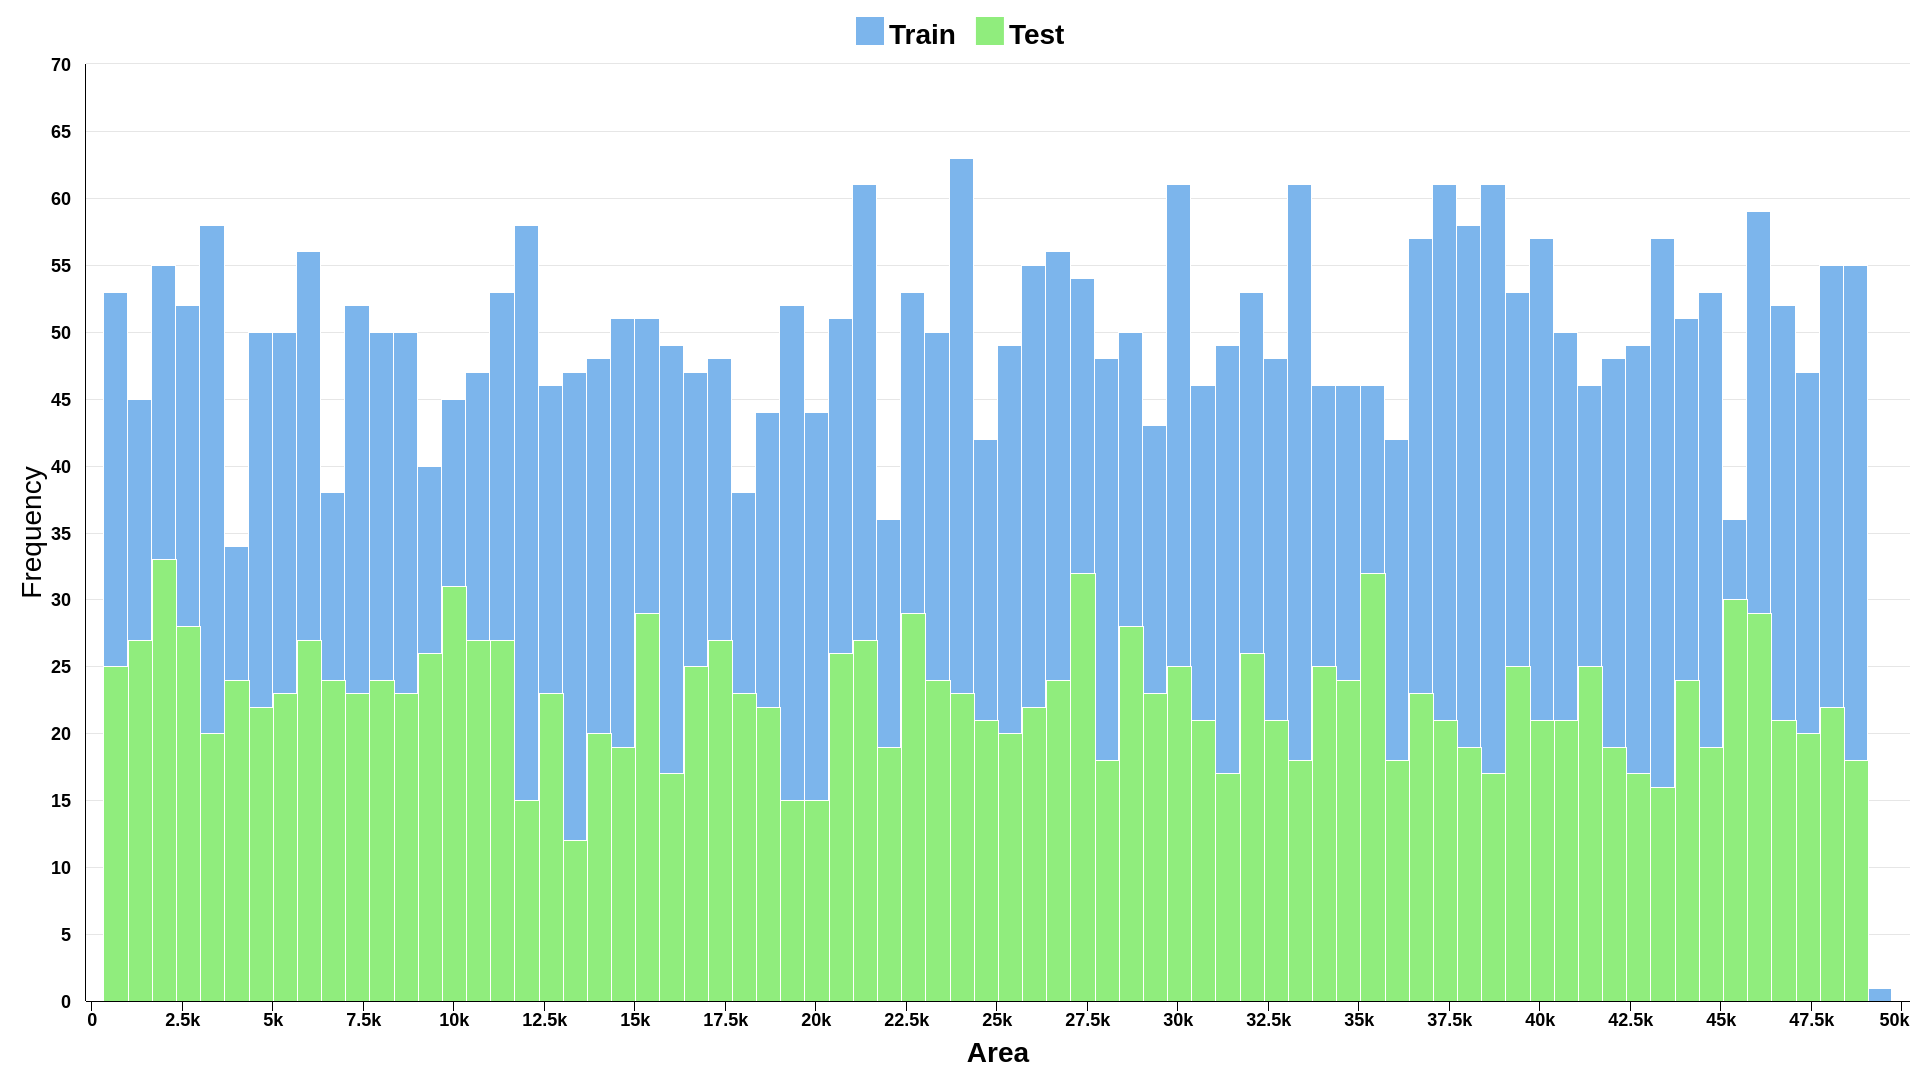
\includegraphics[width=1.0\linewidth]{imgs/Test_9/dataset_9/Circles_Area_Distribution_Hist.png}
        \caption{Distribuição da Área (Circulos)}
        \label{fig:enter-label}
    \end{figure}

\subsection{Treino}

\begin{figure}[H]
    \centering
    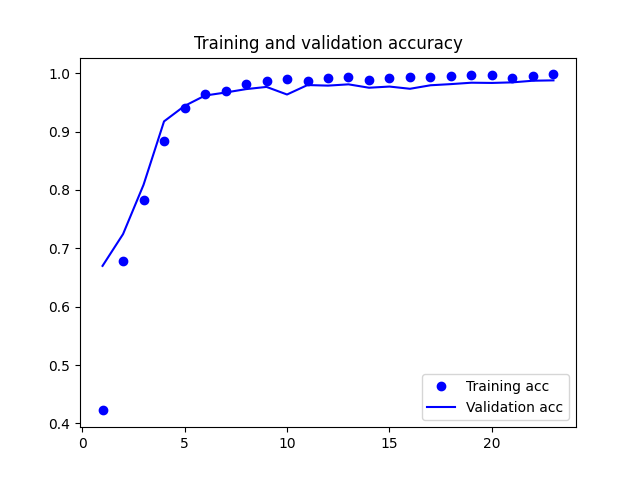
\includegraphics[width=\textwidth]{imgs/Test_9/train_test_acc.png}
    \caption{Acurácia de Validação e de Treino}
    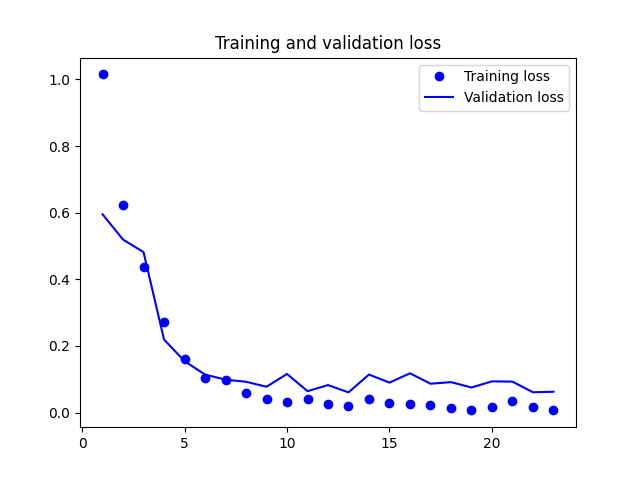
\includegraphics[width=\textwidth]{imgs/Test_9/train_test_loss.png}
    \caption{Perda de Validação e de Treino}
    \label{fig:sub2}
    Com as 23 épocas realizadas, conseguimos uma val acc de 0.9876, sendo que a melhor loss foi atingida na época 13.
\end{figure}

\subsection{Amostras Mal Classificadas}

No total foram mal classificadas 66 (1.32\% ) imagens, sendo 26 (39.39\%) delas circulos, 18 (27.27\%) quadrados e as restantes 22 (33.3\%) vazios. 

\subsection{Matriz de Confusão}

\begin{table}[H]
\centering
\begin{tabular}{l|c c c}
                 & Circulo & Quadrado & Vazio \\
\hline
Circulo          & 2405         & 22     & 1           \\
Quadrado         & 95           & 2330   & 1           \\
Vazio            & 95           & 2330   & 1           \\
\end{tabular}
\end{table}

\subsection{Análise}

\newpage

\section{Teste 10}
\subsection{Objetivo}
    Classificar Imagens com quadrados, circulos e vazios. Ao seja, um problema de classificação não binário.
\subsection{Dataset}
    O Dataset é composto por 10998 imagens de treino e 4998 de teste. Composto por 3 classes: 
    \begin{itemize}
        \item Circulos 
        \item Quadrados
        \item Triangulos
    \end{itemize}
    \begin{figure}[H]
        \centering
        
\includegraphics[width=0.25\linewidth]{imgs/Test_10/dataset_10/circles_9.png}
        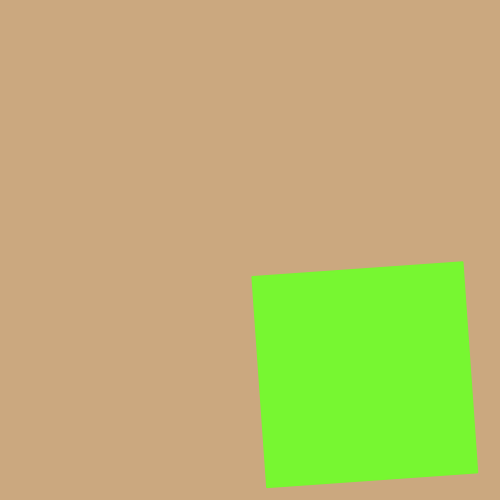
\includegraphics[width=0.25\linewidth]{imgs/Test_10/dataset_10/squares_9.png}
        \includegraphics[width=0.25\linewidth]{imgs/Test_10/dataset_910triangles_9.png}
        \caption{Circlos, Quadrados e Triangulos}
        \label{fig:enter-label}
    \end{figure}
    \begin{figure}[H]
        \centering
        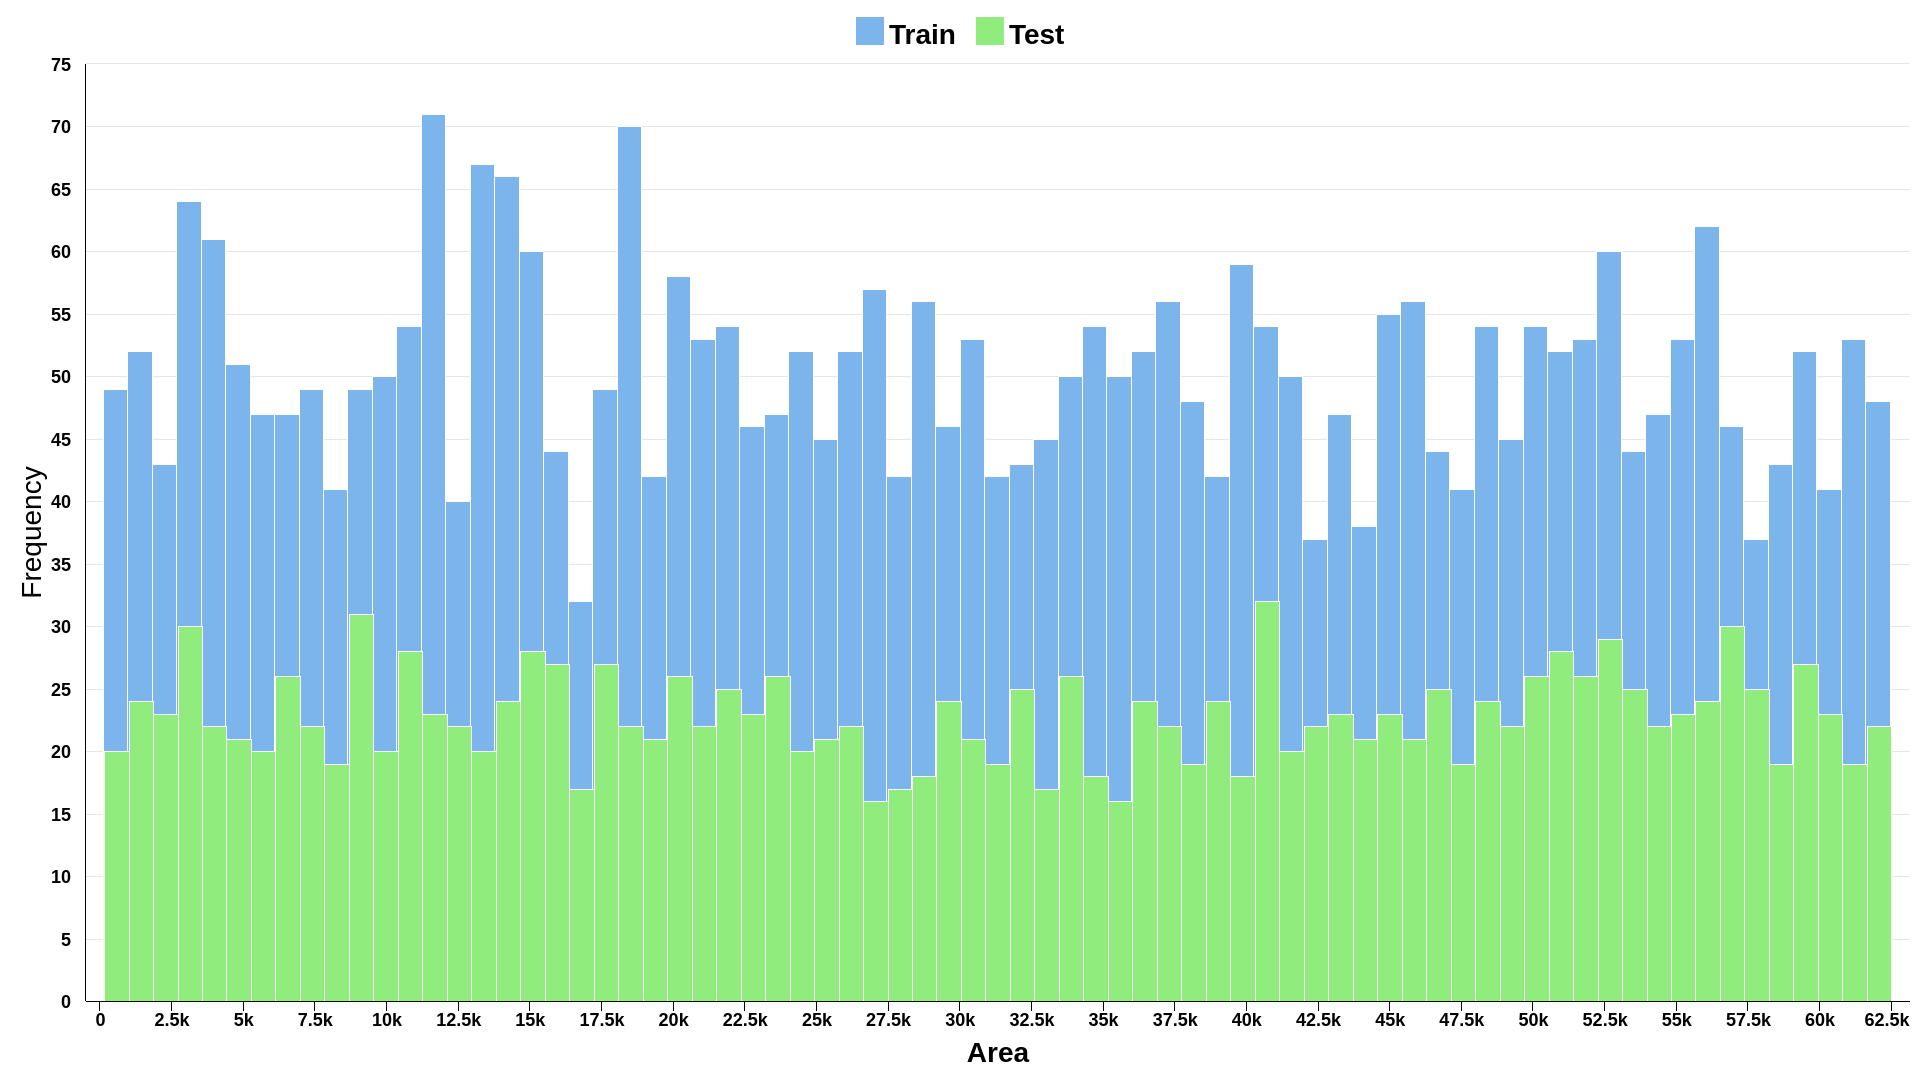
\includegraphics[width=1.0\linewidth]{imgs/Test_9/dataset_9/Squares_Area_Distribution_Hist.png}
        \caption{Distribuição da Área (Quadrados)}
        \label{fig:enter-label}
    \end{figure}
    \begin{figure}[H]
        \centering
        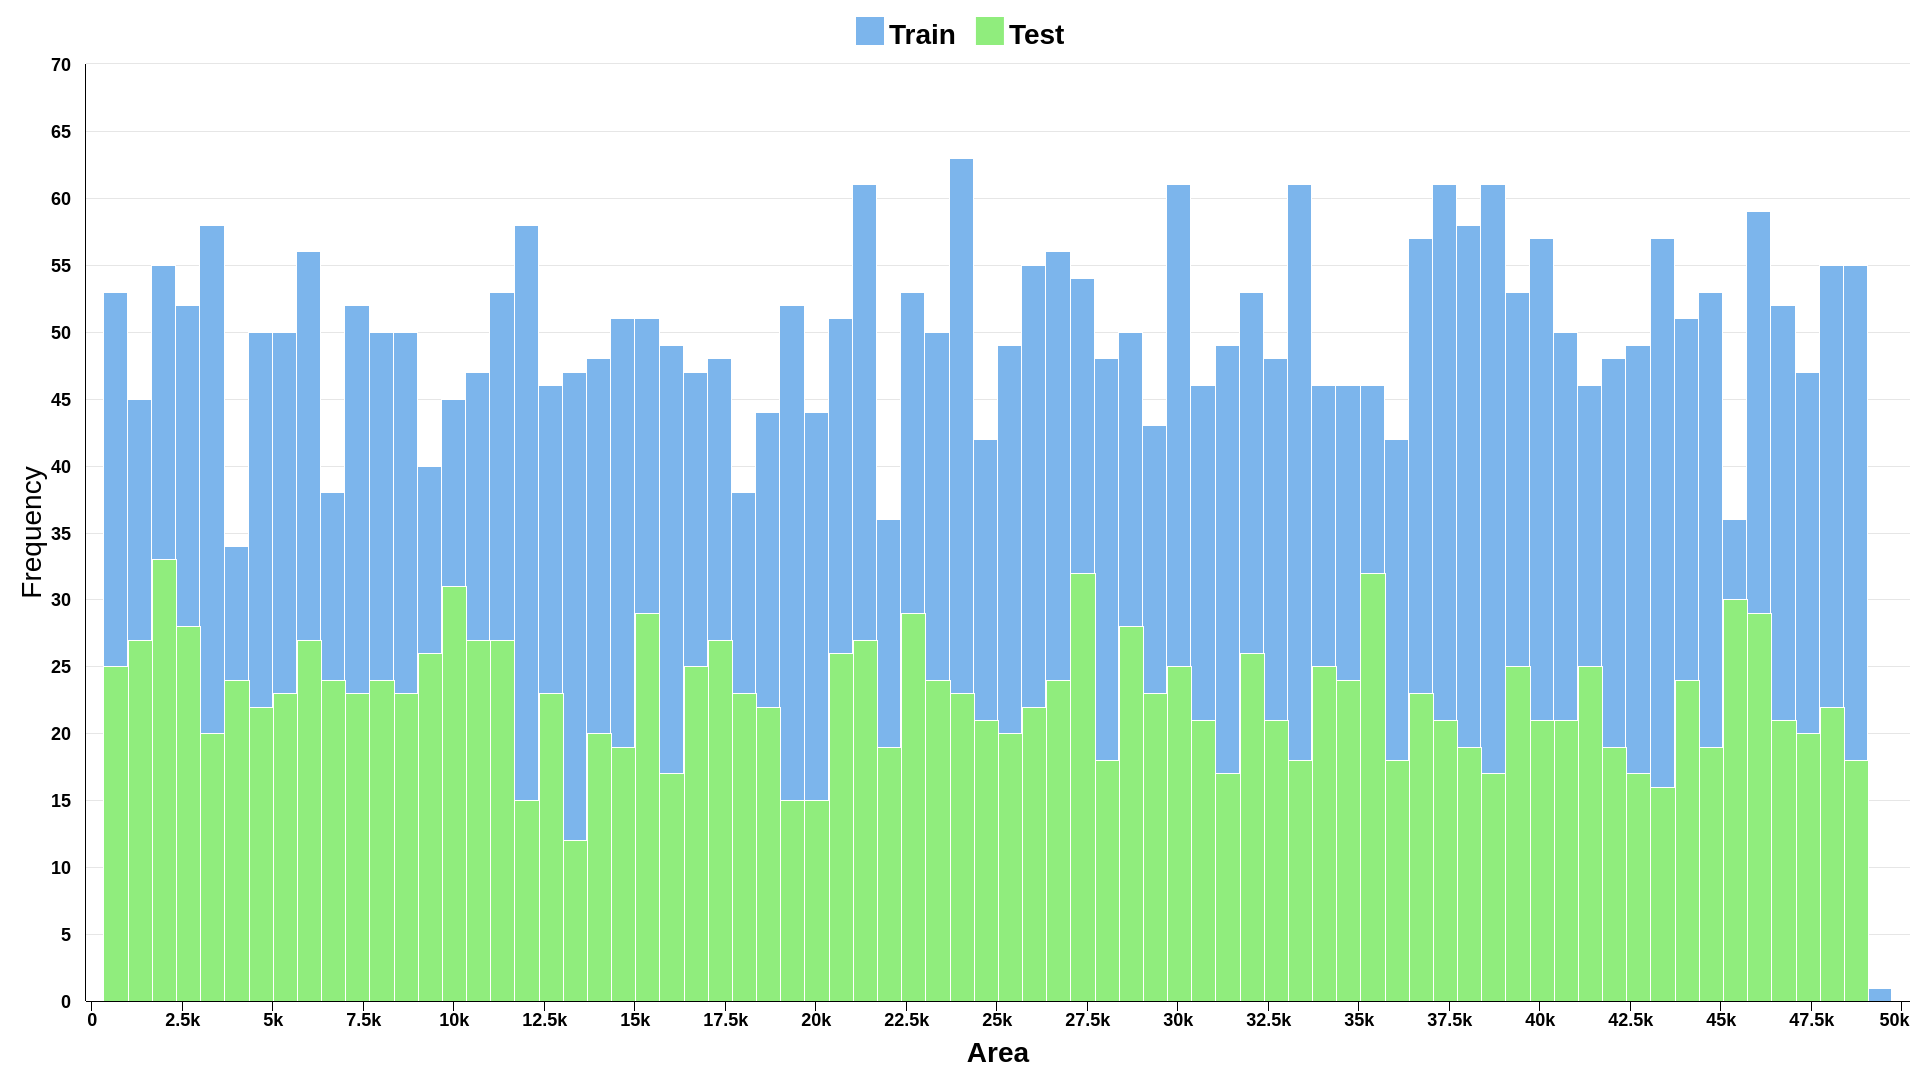
\includegraphics[width=1.0\linewidth]{imgs/Test_9/dataset_9/Circles_Area_Distribution_Hist.png}
        \caption{Distribuição da Área (Circulos)}
        \label{fig:enter-label}
    \end{figure}

\subsection{Treino}

\begin{figure}[H]
    \centering
    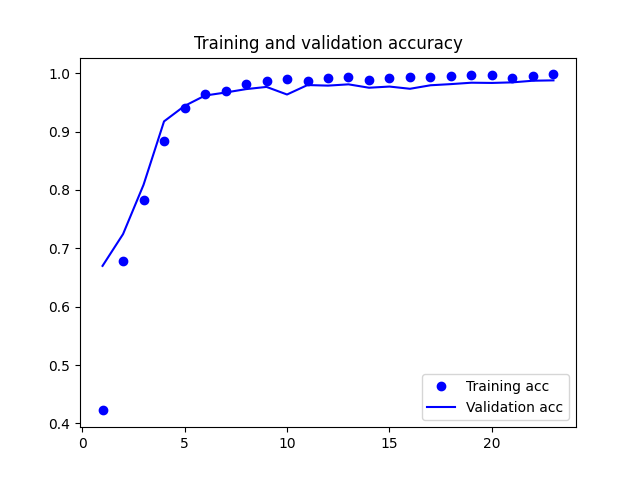
\includegraphics[width=\textwidth]{imgs/Test_9/train_test_acc.png}
    \caption{Acurácia de Validação e de Treino}
    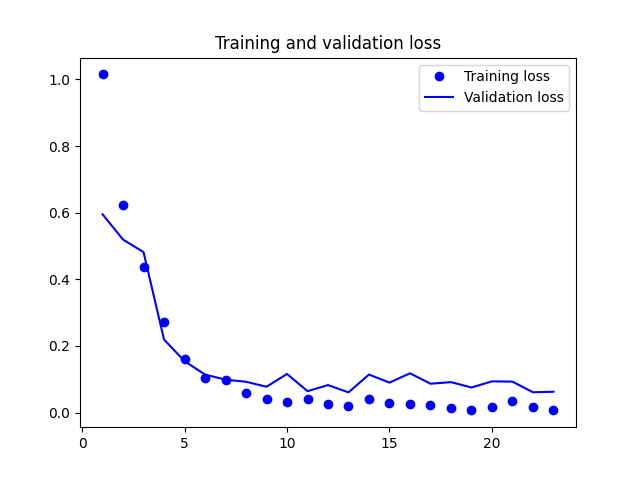
\includegraphics[width=\textwidth]{imgs/Test_9/train_test_loss.png}
    \caption{Perda de Validação e de Treino}
    \label{fig:sub2}
    Com as 23 épocas realizadas, conseguimos uma val acc de 0.9876, sendo que a melhor loss foi atingida na época 13.
\end{figure}

\subsection{Amostras Mal Classificadas}

No total foram mal classificadas 66 (1.32\% ) imagens, sendo 26 (39.39\%) delas circulos, 18 (27.27\%) quadrados e as restantes 22 (33.3\%) vazios. 

\subsection{Matriz de Confusão}

\begin{table}[H]
\centering
\begin{tabular}{l|c c c}
                 & Circulo & Quadrado & Vazio \\
\hline
Circulo          & 2405         & 22     & 1           \\
Quadrado         & 95           & 2330   & 1           \\
Vazio            & 95           & 2330   & 1           \\
\end{tabular}
\end{table}